%%%% ijcai19.tex

%\typeout{IJCAI-19 Instructions for Authors}

% These are the instructions for authors for IJCAI-19.

\documentclass{article}
\pdfpagewidth=8.5in
\pdfpageheight=11in
% The file ijcai19.sty is NOT the same than previous years'
\usepackage{ijcai19}

% Use the postscript times font!
\usepackage{times}
\usepackage{soul}
\usepackage{url}
\usepackage[hidelinks]{hyperref}
\usepackage[utf8]{inputenc}
\usepackage[small]{caption}
\usepackage{graphicx}
\usepackage{amsmath}
\usepackage{booktabs}
%\usepackage{algorithm}
\usepackage{algorithmic}
\urlstyle{same}

%-------------------
\usepackage{times}
\usepackage{helvet}
\usepackage{courier}
\usepackage{amsthm}
%\usepackage{algorithm}

\usepackage{amssymb,amsthm, amsfonts}

\newtheorem{theorem}{Theorem}
\newtheorem{definition}{Definition}
\usepackage[ruled,linesnumbered]{algorithm2e}
\newcommand{\var}{\texttt}

\usepackage{mathtools} % Bonus

\usepackage{lipsum}
\usepackage{csquotes}
\usepackage{verbatim}
\usepackage{tikz}

% \usepackage{multirow}
\usepackage{array,multirow,graphicx}

%% Farbige Kommentar-Felder
%\usepackage[usenames]{color} % Only used in comment commands
%\usepackage{hyperref}
\usepackage{url}
\newcommand{\commentout}[1]{}
\newtheorem{lemma}{Lemma}

\definecolor{Blue}{rgb}{0,0.16,0.90}
\definecolor{Red}{rgb}{0.90,0.16,0}
\definecolor{DarkBlue}{rgb}{0,0.08,0.45}
\definecolor{ChangedColor}{rgb}{0.9,0.08,0}
\definecolor{CommentColor}{rgb}{0.2,0.8,0.2}
\definecolor{ToDoColor}{rgb}{0.1,0.2,1}

\definecolor{verylightgray}{rgb}{0.91,0.91,0.91}

% *** Use this definition of the command to show the meta-info ***
\newcommand{\todo}[1]{\textbf{\color{ToDoColor} TODO: #1}}
\newcommand{\ronen}[1]{\footnote{\textbf{\color{CommentColor} /* #1   (ronen)*/}}}
\newcommand{\raz}[1]{\footnote{\textbf{\color{CommentColor} /* #1  (raz)*/}}}


\newcommand{\generalnote}[1]{#1}

\newcommand{\astar}{\textsc{a*}}
\newcommand{\mafs}{\textsc{mafs}}
\newcommand{\masas}{\textsc{ma-a*}}
\newcommand{\mastrips}{\textsc{ma-strips}}
\newcommand{\strips}{\textsc{strips}}
\newcommand{\hdastar}{\textsc{hda*}}
\newcommand{\cM}{{\cal M}}
\newcommand{\Posp}{\mathit{Pos\mbox{-}p}}
\newcommand{\Negp}{\mathit{Neg\mbox{-}p}}

% the following package is optional:
%\usepackage{latexsym} 

% Following comment is from ijcai97-submit.tex:
% The preparation of these files was supported by Schlumberger Palo Alto
% Research, AT\&T Bell Laboratories, and Morgan Kaufmann Publishers.
% Shirley Jowell, of Morgan Kaufmann Publishers, and Peter F.
% Patel-Schneider, of AT\&T Bell Laboratories collaborated on their
% preparation.

% These instructions can be modified and used in other conferences as long
% as credit to the authors and supporting agencies is retained, this notice
% is not changed, and further modification or reuse is not restricted.
% Neither Shirley Jowell nor Peter F. Patel-Schneider can be listed as
% contacts for providing assistance without their prior permission.

% To use for other conferences, change references to files and the
% conference appropriate and use other authors, contacts, publishers, and
% organizations.
% Also change the deadline and address for returning papers and the length and
% page charge instructions.
% Put where the files are available in the appropriate places.

\title{Multi-Agent Path Finding under Uncertainty and Uncontrollability}

% Single author syntax
\author{
    	Authors
    	\affiliations
    	ABC Institute
  	\emails
    	xyz@ijcai19.org
}

% Multiple author syntax (remove the single-author syntax above and the \iffalse ... \fi here)
% Check the ijcai19-multiauthor.tex file for detailed instructions
\iffalse
\author{
First Author$^1$
\and
Second Author$^2$\and
Third Author$^{2,3}$\And
Fourth Author$^4$
\affiliations
$^1$First Affiliation\\
$^2$Second Affiliation\\
$^3$Third Affiliation\\
$^4$Fourth Affiliation
\emails
\{first, second\}@example.com,
third@other.example.com,
fourth@example.com
}
\fi

\begin{document}

\maketitle

\begin{abstract}
In many real-world scenarios, the time it takes for a mobile agent, \emph{e.g.}, a robot, to move from one location to another may vary due to exogenous events and cannot be accurately predicted upfront. This poses a significant challenge especially when planning paths for multiple agents, since temporal coordination is necessary in order to avoid collisions. The problem becomes much severe when an agent is not sure about definite initial and goal locations of other agents during plan execution. 
Each agent maintains a pair of belief states that capture uncertainty over initial and goal states, for each of the remaining agents.  
In this work, we address these challenges of path planning for multiple agents when there is uncertainty over action duration, and their initial and goal states. 
We propose two new algorithms to solve this variant of MAPF problem. They are respectively based on the Conflict-Based Search and $\mathrm{A^{*}+OD}$ algorithms. 
They are offline algorithms that strive for a \emph{strong solution} that consists of one plan for each agent that is guaranteed to reach their goal safely under given uncertainty. 
We prove the soundness, completeness, and optimality \emph{w.r.t.} various optimality measures, of the proposed algorithms, and demonstrate its applicability on standard multi-agent pathfinding domains.  
\end{abstract}

\section{Introduction}
In a Multi-Agent Path Finding (MAPF) problem, paths are found for multiple agents where each agent has different start and goal positions, such that the agents do not collide while executing their obtained paths in a distributed manner (without communication). 
MAPF problems arise for aircraft towing vehicles~\cite{MorrisPLMMKK16}, video game characters~\cite{Silver05}, office robots~\cite{VelosoBCR15}, and warehouse robots~\cite{WurmanDM07}, among several other scenarios.

Many recently proposed MAPF solvers scale to large MAPF instances~\cite{SharonSFS12,FelnerLB00KK18}. However, they are based on some assumptions that are less realistic, for example: 1. agents are always \emph{certain} about their starting positions; 2. a \emph{finite} time is required to travel a path between two locations; 3. their goal locations are definite too. 
In a more realistic setting, during distributed plan execution an agent cannot always be sure about other agents' initial locations, effects of actions they perform -- known as non-deterministic action effect (for ease of exposition we only consider a non-deterministic action execution time), and their goal locations.  
There is a well researched sub-area of AI Planning known as conformant planning~\cite{HoffmannB06,PalaciosG09}, which is closely related to this.
Conformant planning is the task of generating plans given uncertainty about the initial state and action effects, and without any sensing capabilities during plan execution. The plan should be  successful regardless of which particular initial world we start from.

Often to predict accurately the exact required time for an agent to travel a path in the real world is impossible. This uncertain travel time lies in some time range, \emph{e.g.}, $[T_{min}, T_{max}]$ that is provided by an oracle.  
%%
%A \emph{time} required to traverse an edge (a path) can be uncertain too. 
%%
Moreover that, sometimes, the plan executor cannot control the execution as well, which means, once an agent starts travelling through that path, only nature can decide the finish time, $f_T$, \emph{s.t.}, $T_{min} \leq f_T \leq T_{max}$.
%
For example, a robot might take more (or less) time to travel from one place to another,  depending on the external conditions such as slippery floor or path blockage. 
Further, an agent might be certain \emph{only} about its own goal state but uncertain about other agents' goal states~\cite{BolanderEMN18}.
Perhaps an agent is certain about a set of possible goal locations for all the remaining other agents. 
Table~\ref{tab:tab1} captures details of possible uncertainty  we propose to handle in MAPF setting, during the planning and execution phases. 
The planning is fully centralized and offline while the plan execution is fully distributed with no communication.

\begin{table}[]
    \centering
    \begin{tabular}{| l | c | c | c | c |}
    \hline
        \multirow{2}{*}{\multicolumn{1}{c}{\textbf{Uncertainty}}} &  \multicolumn{2}{c|}{\textbf{Planning}} & \multicolumn{2}{c|}{\textbf{Execution}} \\ 
    %\cline{2-5}
        & \emph{Self} & \emph{Others} & \emph{Self} & \emph{Others} \\ 
    \hline
        \emph{Start state} & U & U & P & U \\
    %\hline
        \emph{Goal state} & U & U & P & U \\
    %\hline
        \emph{Traversal time} & U & U & U & U \\
    \hline
        \multicolumn{1}{|c|}{\textbf{Approach}} 
        & \multicolumn{2}{c|}{\emph{Centralized}} & \multicolumn{2}{c|}{\emph{Distributed}} \\
    \hline
    \end{tabular}
    \caption{The notion of \emph{uncertainty} and \emph{partial observability} in planning and execution phases for an agent is shown, where U -- uncertainty and P -- perfect information. For example, during the execution an agent (\emph{Self}) has fully aware of its own initial and goal states but uncertain about other agents' (\emph{Others}) state details.}
    \label{tab:tab1}
\end{table}

Although we introduce uncertainty in MAPF setting, our high-level goal still remains the same as in CBS~\cite{SharonSFS12} or $\mathrm{A^*}$ with Operator Decomposition (OD)~\cite{Standley10}, which is that all agent should reach their any individual specific goal positions from their specific starting positions optimally without any collision. 
We propose two \emph{centralized} + \emph{offline} algorithms to tackle such MAPF problems. 
Each algorithm generates  \emph{strong} solutions~\cite{CimattiDMRS18} that are optimal and guaranteed to be collision free under given uncertainty. 
However, to solve such problems one can use \emph{online} approaches for each agent under certain assumptions about their initial states, goal states, and edge traversal times. 
This would often lead to a runtime-intensive replanning or plan-execution failures~\cite{0001KK17}. Agents might have scenarios where the centralized planner would not have enough time to replan for each agent online~\cite{CimattiDMRS18}. 
Further, agents need a communication channel between themselves and the centralized solver to communicate their current state and (or) reason of failure etc. Establishing any such communication channel is costly and it can also be broken during execution. 
%
%; those scenarios, an obtained solution must be mph{robust}~\cite{AtzmonSFWBZ18} to all possible execution time uncertainty. A robust solution is also known as \emph{strong} solution~\cite{CimattiDMRS18}.

%For an effective plan execution we assume that when an agent finalizes its  conformant-path, an oracle provides it with the knowledge of its true initial state. However, the time uncertainty on the edges remains the same during the execution too. \todo{Can we say this? We take one possible state from $b_0^{i}$, for each agent, find plans. Now we know their real initial states. The best case is that they were their true initial states. The worst case to find a completely new set of plans for the true initial states.} 

% We formally describe important terms like \emph{UTB} and \emph{LTB} that respectively stand for Upper Time Bound and Lower Time Bound, in the later part of the paper.
%

We propose two algorithms to solve this MAPF problem. 
The first algorithm is called \textbf{C}onformant \textbf{C}onflict \textbf{B}ased \textbf{S}earch under \textbf{T}ime \textbf{U}ncertainty (\textbf{CCBSTU}), which is solely based on CBS~\cite{SharonSFS12}. 
It is a continuum of coupled and decoupled approaches.
%
%
Abstractly, CCBSTU is a two-level algorithm, where at the \emph{top-level} a search is performed in a Constraint Tree (CT). 
Nodes of CT include constraints on time and location for a single agent. A location in the graph $G = (V,E)$, could be an edge $e \in E$ or a vertex $v \in V$. 
At \emph{bottom-level} a search is performed at each node of the constraint tree.
For each agent, it generates a new path using CCBSTU such that they satisfy the constraints imposed on the agent by the high-level CT node.  
%
The second algorithm is called 
\textbf{C}onformant ${A}^*$ with  
\textbf{O}perator \textbf{D}ecomposition under \textbf{T}ime 
\textbf{U}ncertainty (\textbf{CAODTU}) that is based on $A^*$ with OD~\cite{Standley10}. 
In this algorithms a standard operator is decomposed into series of operators. 
We prove that our proposed algorithms are sound and complete, and solutions obtained through them are always optimal.

The rest of the paper is structured as follows. We begin with our overall problem statement followed by a brief background on CBS algorithm and other related work. We then discuss a general approach to find and resolve a conflict when the problem has uncertainty only about the edge traversal time. 
This is used in CCBSTU algorithm. We describe how the CAODTU algorithm works under time uncertainty. This is followed by detailed descriptions of the CCBSTU and CAODTU algorithms for the MAPF problem under uncertainty covered in this section. 
Later, we study these algorithms theoretically followed by their empirical evaluations and their comparison on several new standard problems. We conclude with a summary and future work.

\section{Problem Statement}
The problem we address in this paper is fundamentally a variant of the classical MAPF problem~\cite{SharonSFS12}. We provide a detailed description of a high-level problem that has been tackled in this work.

There is a given graph, $G = (V,E)$, and a set of $k$-agents labeled $a_1,\ldots,a_k$. Being uncertain about its initial and goal locations during planning, each agent $a_i$ maintains initial and goal belief states, $b_I^{a_i}$ and $b_g^{a_i}$, respectively, such that $b_I^{a_i} \subseteq V$ and $b_g^{a_i} \subseteq V$. 
For the simplicity, we consider that agent's moves make only deterministic changes that are fully observable. It is trivial to extend our approach to handle non-deterministic action effects. 
For example, in a grid an agent takes a move in the \emph{east} direction might slide to the location \emph{south} to its current location because of slippery floor. However, we consider the case where an agent can take an uncertain amount of time (a \emph{natural number} in $[T_{min}, T_{max}]$) to traverse an edge $e \in E$ in either direction. This time frame is provided by some \emph{oracle}.
%
On each clock tick an agent either \emph{waits} -- remains at its location, or \emph{moves} towards a neighboring location, traversing the edge $e$. In the latter case, it either occupies $e$ or the destination in the next time tick. 
%
%We consider that an edge or a vertex of a graph as a resource that can be provided to at most one agent at a time. 
%
%We assume that for each edge there is an \emph{oracle} that gives us its traversal time frame, $[T_{min}, T_{max}]$. 
%
The time required during execution to traverse this edge lies within this time frame including the boundary values.
The finish time ($f_T$) however cannot be determined by the plan executor on its own; and can only be determined by nature at run time.
We assume that at most one agent can occupy a vertex $v \in V$ or an edge $e \in E$ at an instant $t$.  

The task is to return a set of paths $\Pi_{a_i}$ for an agent $a_i$, considering each location $l \in b_I^{a_i}$ as a possible initial location and each location $g \in b_g^{a_i}$ as a possible goal location, consequently, $|\Pi_{a_i}| \leq |b_I^{a_i}| \times |b_g^{a_i}|$. 
Basically, a possible initial state of $a_i$ can be its possible goal state too. To find a collision free set of paths, for any two agents the sets of their possible initial locations and the goal locations must be disjoint.
For each plan $\pi_{a_i}^{l} \in \Pi_{a_i}$ there exists no conflicts between $\pi_{a_i}^{l}$ and each valid plan $\pi \in \Pi_{a_j}$, for all the other agents $a_j$. 
We \emph{optimize} the approach over some standard parameter in the process. In the experiments, we optimize on the earliest time an agent could reach the goal location, is denoted as a cost function as $C$ that is equal to $\sum_{a_i \in \{a_1...a_k\}} \sum_{\pi \in \Pi_{a_i}} \mathit{LTB}(\pi)$. 
%
$\mathit{LTB}(\pi)$ stands for \emph{lower time bound}: the minimum time an agent takes to reach its goal following its plan $\pi$.
On the other hand, even if the agents have full information about their initial and goal locations  then uncertainty only lies in edge traversal time. Still, our overall task remains the same. The only difference is that now each agent $a_i$ finds a single collision free path as $|b_I^{a_i}| \times |b_g^{a_i}| = 1$.

\section{Background and Related Work}
\todo{
\subsection{Conflict Based Search}
Conflict Based Search (CBS)~\cite{SharonSFS12}... 
%
\subsection{MAPF under Time Uncertainty}
How would CBS look like if the MAPF problem is considered under temporal Uncertainty...}
%

\begin{figure}[ht]
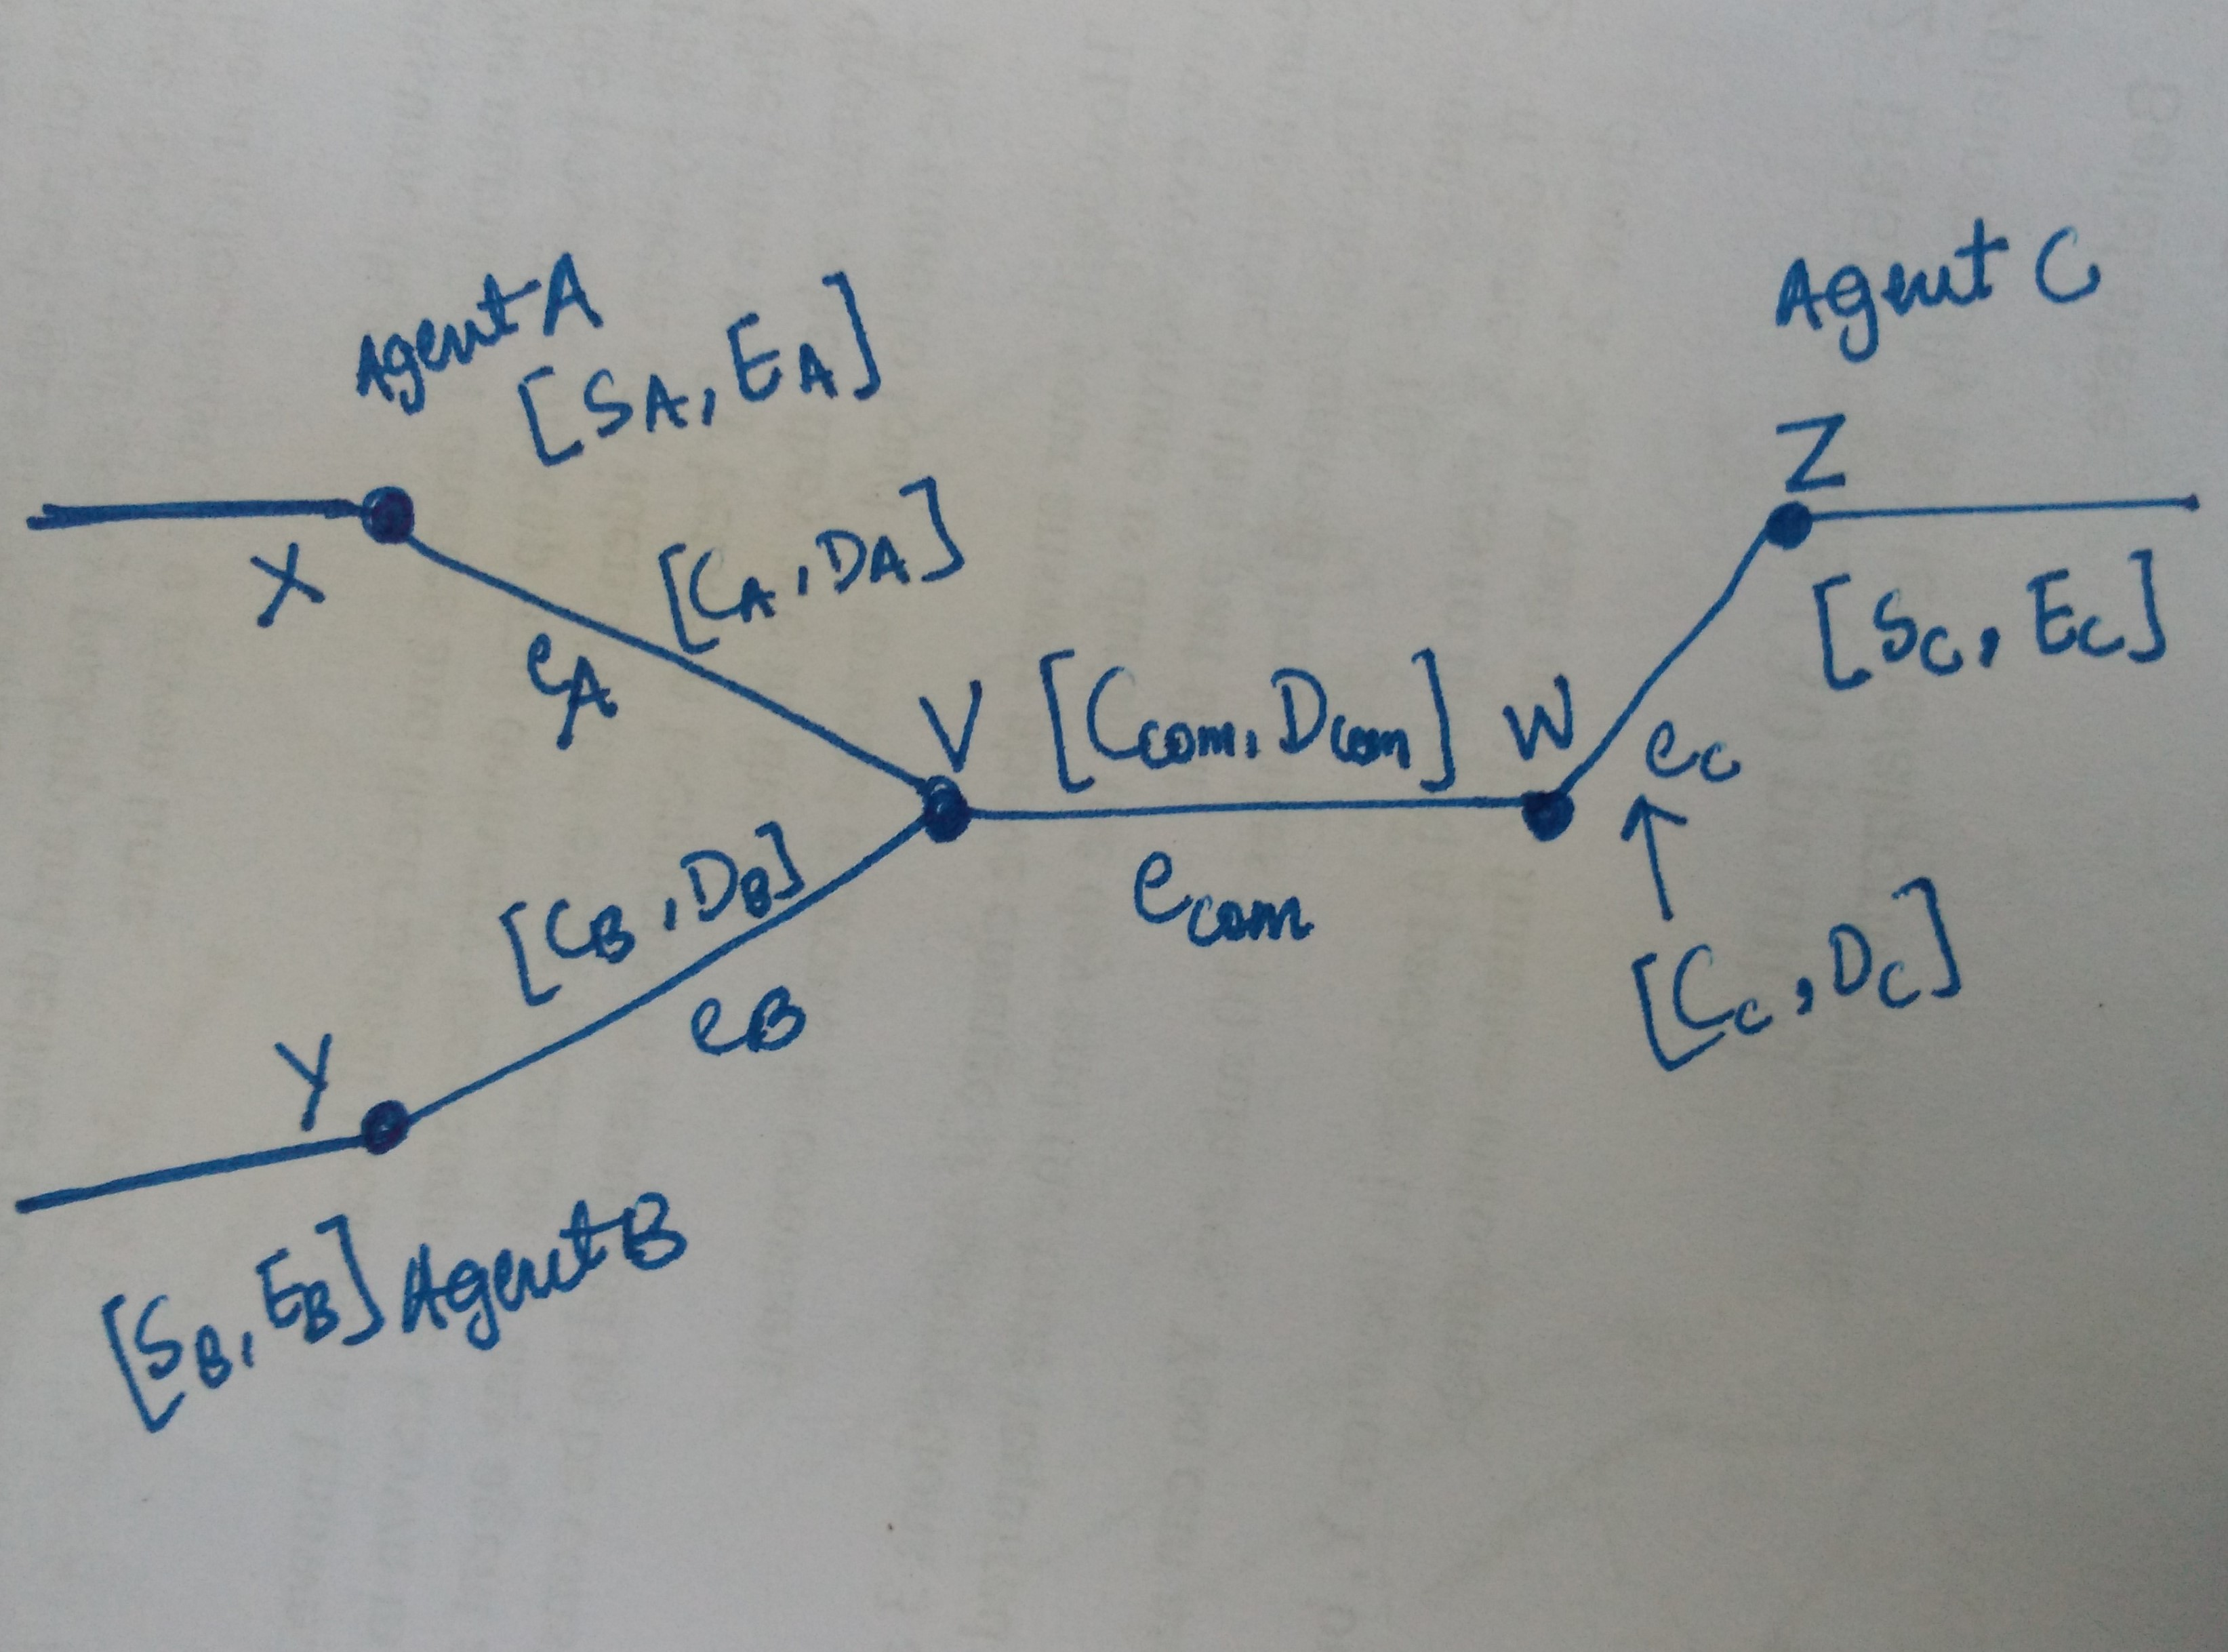
\includegraphics[width=8.5cm,height=6cm]{img11.jpg}
\caption{Captures three agents A, B and C for the motivated MAPF problem. The description of our approach is based on this diagram. 
%
%(\textcolor{blue}{\todo~Draw this graph properly, though the characters and notations used would remain the same.})
}
\label{fig:1}
\end{figure}

\section{MAPF under Time Uncertainty}
We start with a MAPF problem that posses uncertainty only about traversal time. Based on the CBS algorithm, we first thoroughly describe a general approach of finding and resolving a conflict which is used to describe CCBSTU, our first algorithm, later. 
We then describe our second algorithm based on the general $\mathrm{A^* + OD}$ algorithm to handle only time uncertainty in this setting. In the next section, they are generalized to a case when agents have uncertainty over their initial and goal states.

\subsection{Finding and Resolving a Conflict}
We show an example scenario in Figure~\ref{fig:1}.
There are three agents A, B and C, and they occupy vertices X, Y and Z, respectively. $[S_A,E_A]$ indicates the start and end time agent A could possibly occupy vertex X, similarly for agents B and C for the vertices Y and Z, respectively. 

%\subsection{Action Conflict}
%We propose a new type of conflict called an \emph{action conflict}.
Current actions or moves of two agents are \emph{conflicting} if, in the next clock tick, they could possibly occupy the same vertex or edge together which is restricted. 
Our approach of finding and resolving such conflicts, is an adaptation of the approach used in CBS algorithm. 
%Whilst such pair of actions are known as conflicting actions.   

\subsubsection{Vertex Conflict}
Consider a case when two agents could possibly occupy a vertex simultaneously by applying a conflicting pair of moves. In Figure~\ref{fig:1}, agent A could reach V at $T_A = [S_A+C_A, E_A+D_A]$, and agent B could reach V at $T_B = [S_B+C_B, E_B+D_B]$. Their individual moves cause a \emph{vertex conflict} if $T_A \cap T_B \neq \phi$. Assume that, $[t_1,t_2]$ is the intersection of $T_A$ and $T_B$, which is a common time frame in which A and B occupy vertex V, simultaneously. 
%We define this as \emph{action conflict} and can be found for given two agents' plans. 
A vertex conflict is represented as: $(A,T_A,B,T_B,V)$ that reads as agents A and B reach V at $T_A$ and $T_B$ respectively such that $T_A \cap T_B \neq \phi$.

CBS resolves such conflicts by constraining one of the agents such that it does not occupy vertex V at a time instance. 
Following that an easy solution for our case is to just restrict one of A and B to occupy V in $[t_1,t_2]$.
If we deal with time intervals, this naive solution makes our algorithms incomplete. The approach could easily miss out an only possible solution due to such strong restriction. 
For example, consider that $[S_A,E_A] = [0,0]$ and $[S_B,E_B] = [0,0]$ in Figure~\ref{fig:1}. The time ranges for the edges XV and YV are $[C_A,D_A] = [5,11] \text{ and } [C_B,D_B] = [7,18]$, respectively.
%%
Assume that there are two more edges XV and YV having the time ranges of $[8,9] \text{ and } [9,10]$ respectively. If the search minimizes 
LTB, the algorithm would place a strong constraint, $[t_1,t_2] = [7,11]$, on the vertex $V$ in the first go. 
Therefore at least one agent is not allowed to occupy $V$ in $[7,11]$ in all possible solutions.
%This strong constraint guarantees that the approach would miss the only possible solution. 
The agents are not allowed to move via other two edges XV and YV.
%%
Similarly we can also guarantee that sometimes even restricting an agent for two consecutive  clock ticks, $t$ and $t+1$, such that $t$ and $t+1$ belong to $[t_1,t_2]$, makes the approach incomplete.   

Given a vertex conflict, we know that in any valid solution at most one of A and B can occupy V in $[t_1,t_2]$.
We \emph{resolve} it by constraining only one agent at a time, such that it cannot occupy V at an arbitrary $t \in [t_1,t_2]$. Therefore, at least one of the constraints, which are $occupy(A,V,t)$ and $occupy(B,V,t)$ \emph{s.t.} $t \in [t_1,t_2]$, must be added to the set of constraints. 
A constraint, $occupy(A,V,t)$, specifies that agent A is not allowed to occupy vertex V at time $t$. In other words, A is not allowed to take a move such that it can reach V at $[t_l,t_m]$ and $t \in [t_l,t_m]$. 
%Note that we choose $t$ in an arbitrary manner.
We examine both possibilities to guarantee the solution optimality, which means that current CT node splits into two two children nodes. 
Both children inherit the constraints from the parent node. 
Moreover, the left child receives a new constraint $occupy(A,V,t)$ and the right child receives $occupy(B,V,t)$.         

% In one solution For the interval $[t_1,t_2]$, constraints on agent A are imposed and described as follows. Suppose, $t$ is the time when A and B occupy V simultaneously. One way to resolve this by restricting A using a constraint: {$(\neg move(A,e_A,t-D_A) \wedge \neg move(A,e_A,t-(D_A-1)) \wedge ... \wedge \neg move(A,e_A,t-C_A))$. Here, each component $\neg move(A,e_A,t_x)$ represents that A is not allowed to apply move action through edge $e_A$ at time $t_x$. Consequently, the conjunction removes all the possibilities for agent A occupying vertex V at time $t$. 
% For example, if A applies \emph{move} at $t-D_A$, at the earliest it can reach V by $t-D_A+C_A$ and late by $t$. Similarly, if A applies \emph{move} at $t-C_A$, at the earliest it can reach V by $t$ and late by $t-C_A+D_A$, and so on for intermediate values between $t-D_A$ and $t-C_A$. In all these cases there is possibility that A can occupy V at $t$. We generalize this approach for all $t \in [t_1,t_2]$. 
% This generalization under uncertainty and uncontrollability restricts A, following its current path, to occupy V in the interval $[t_1,t_2]$ in any situation that could occur, consequently allows agent B to execute its current plan as it is. 
% On the contrary, we can allow A to execute its current plan by restricting B in exactly the same way. This approach produces sound solutions as well as it is complete, and their proofs are formally covered later in the paper. 


\subsubsection{Edge Conflict} Uncertainty and uncontrollability help arise two types of \emph{edge conflicts} given our MAPF settings. 
In Figure~\ref{fig:1}, when A and B traverse the edge $e_{com}$ from V to W in which one agent might \emph{run-over} the other or possibly occupy $e_{com}$ simultaneously. 
The other scenario is when the agents have \emph{head-on} collision while they traverse this edge in the opposite directions at the same time. 

\noindent \textbf{First Case.} 
Assume that there is no vertex conflict at V such that A occupies V at $[S_A+C_A,E_A+D_A]$ while B occupies V at $[S_B+C_B,E_B+D_B]$ (Figure~\ref{fig:1}). 
They traverse the common edge $e_{com}$ from V to W, and reach W respectively at $[S_A+C_A+C_{com},E_A+D_A+D_{com}]$ and $[S_B+C_B+C_{com},E_B+D_B+D_{com}]$. 
%
This type of edge conflict is only possible if $D_{com} \geq 2$ otherwise no need to look for such conflicts. 
We assume that $D_{com} \geq C_{com} \geq 1$ and $D_{com} \geq 2$. Here, agent A could possibly occupy $e_{com}$ in the interval $T_A = [S_A+C_A+1,E_A+D_A+D_{com}-1]$.
Agent A can be on the edge from time $S_A+C_A+1$ up to $E_A+D_A+D_{com}-1$.  Considering all uncertainty and uncontrollability it is bound to reach W by at most $E_A+D_A+D_{com}$.
Similarly for agent B, where it could possibly occupy the edge at $T_B = [S_B+C_B+1,E_B+D_B+D_{com}-1]$.
%
Following the previous approach we compute $[t_1,t_2] = T_A \cap T_B$. If the intersection is non-empty, there is an edge conflict, which means,  A and B possibly occupy $e_{com}$ together.
%
The conflict is represented as: $(A,B,e_{com},[S_A+C_A,E_A+D_A],[S_B+C_B,E_B+D_B], [C_{com},D_{com}])$. 
Note that if an agent starts moving through $e_{com}$ at $t_k$ then at $t_{k}+1$ it can occupy the edge or reach the other end of the edge depending on the time uncertainty. 
It is also possible that it can keep $e_{com}$ engaged until $t_k+D_{com}-1$.

Based on how a vertex conflict is resolved in our MAPF framework, to \textit{resolve} this type of an edge conflict, we must restrict one of the agents to occupy $e_{com}$ at $[t_1,t_2]$. 
Simply restricting agents for whole $[t_1,t_2]$ would make the algorithm incomplete, e.g., a situation exactly like the one we provide with for the vertex conflict case.
%%
Therefore one way to resolve this is by restricting A with a constraint: $occupy(A,e_{com},t)$ where $t \in [t_1,t_2]$. The constraint specifies that A is not allowed to occupy edge $e_{com}$ at $t$. 
Similarly, B can be restricted using the constraint: {$occupy(B,e_{com},t)$ s.t. $t \in [t_1,t_2]$. To guarantee solution optimality we examine both these possibilities. 

\noindent \textbf{Second Case.} A bit complex case compared to the the first one as some subtle issues might arise, is defined as \emph{head-on} collision -- when two agents traversing an edge in opposite directions simultaneously. 
A simple case is, which is also easy to detect, when two agents traverse an edge in opposite directions and they possibly occupy the edge together at $[t_1,t_2]$, computed in a similar manner. 
For example, in Figure~\ref{fig:1}, agent A reaches V at $[S_A+C_A,E_A+D_A]$ and another agent C reaches W at $[S_C+C_C,E_C+D_C]$, and they traverse in the opposite directions. Agent A could occupy $e_{com}$ at $T_A = [S_A+C_A+1,E_A+D_A+D_{com}-1]$ while agent C could occupy it at $T_C = [S_C+C_C+1,E_C+D_C+D_{com}-1]$. 
There is an edge conflict if $[t_1,t_2] = T_A \cap T_C \neq \phi$. 
Moreover, this conflict is also possible when $T_A \cap T_C = \phi$ under some conditions. 
For example, when A reaches V at $[3,3]$ and C reaches W at $[3,3]$, and $[C_{com},D_{com}] = [1,1]$. Following Figure~\ref{fig:1}, this case is only possible when $S_A+C_A = E_A+D_A$, $S_C+C_C = E_C+D_C$ and $C_{com}=D_{com}=1$. In any other situation than this, assuming that $D_{com} \geq C_{com} \geq 1$, there is a proper edge conflict where agents can occupy the edge for some time interval. The conflict is represented in a similar way, $(A,C,e_{com},[S_A+C_A,E_A+D_A],[S_C+C_C,E_C+D_C], [C_{com},D_{com}])$. We do not need to mark the direction of movement of an agent as time intervals in the representation suffice. 

We resolve this conflict in the same way we resolve a run-over conflict. Generates two new children with two new constraints $occupy(A,e_{com},t)$ and $occupy(C,e_{com},t)$ respectively for agents A and C. They inherit all the parent's constraints. 
%
% To resolve conflicts of this kind, we restrict, at least, one of A and C to start its current move at \emph{time} that possibly enables the agent to occupy $e_{com}$ at an instance $t \in [t_1,t_2]$. 
% Following our previous description, first we restrict A using the constraint {$(\neg move(A,e_{com},t-1) \wedge \neg move(A,e_{com},t-2) \wedge ... \wedge \neg move(A,e_{com},t-(D_{com}-1))$. Similarly, in the second approach we restrict B using the constraint {$(\neg move(B,e_{com},t-1) \wedge \neg move(B,e_{com},t-2) \wedge ... \wedge \neg move(B,e_{com},t-(D_{com}-1))$, for all $t \in [t_1,t_2]$. 
%To guarantee optimality both these possibilities are examined. 
%This captures all possible scenarios that could ever cause a head-on collision.
%
We can resolve a collision when they are likely to occupy an edge simultaneously, but this approach cannot capture a case when $T_A \cap T_C = \phi$. 
To resolve this special type of edge conflict, again two children are generated and are explored to guarantee solution optimality.
Left child restricts agent A by $occupy(A,e_{com},(S_A+C_A + C_{com}/2))$, and in the right C is restricted by $occupy(C,e_{com},(S_C+C_C + C_{com}/2))$. Note that, $(S_A+C_A + C_{com}/2) = (S_C+C_C + C_{com}/2)$. The children directly inherit all the parent's constraints. 
%
% First restrict A using $move(A,e_{com},S_A+C_A)$, and in the other solution restrict C using $move(C,e_{com},S_C+C_C)$.   
We are not over constrained with this approach of resolving a head-on conflict and hence do not miss out on any possible solution, consequently, preserving the completeness.

The above discussed approaches to resolve various kind of conflicts, guarantee that we do not loose the completeness. 
We always return a valid solution if there exists one. 
However, we do suspect that there would be some optimistic way to choose $t \in [t_1,t_2]$ instead of an arbitrary, or rather two or more contiguous $t$'s after some preprocessing of the given problem graph. 
This probably would not improve the worst case theoretical guarantees discussed later in the paper, but could improve things practically.  

%%%old section
\subsection{CBS under Time Uncertainty}
\label{cbstu}
The state-space of Multi-Agent Path Finding (MAPF) is exponential in the number of agents.
In the single-agent case, search-space grows only linearly in the graph size.
CBS solves a MAPF problem by decomposing it into a large number of single-agent path finding problems.

In the basic CBS algorithm, an agent takes exactly one unit of time to reach a state connected to their current state (Sharon et el., 2012). We consider that to traverse an edge, e.g., moving from location A to location B, an agent takes a non-deterministic time $t \in [T_{min}, T_{max}]$, where $t$ is decided by the nature at run time. We adapt and improve the technicalities of the basic CBS algorithm to handle this novel setting. 
We first deal with only time uncertainty with perfect information about initial state and goal state. Therefore we skip the \emph{conformant} part from CCBSTU and describe CBSTU first. 

% The next two sub-subsections elaborate upon the approach, based on CBS, to find a pair of conflicting path and to resolve them, 
% when a non-deterministic and uncontrollable edge traversal finish time is considered. First we discuss a general approach to find edge and vertex conflicts and how to resolve them. This approach is employed by CBSTU and CCBSTU that extends CBSTU.   

% % %%%%
% % \begin{figure}
% % \begin{tikzpicture}[sibling distance=9.5em,
% %   every node/.style = {shape=rectangle, rounded corners,
% %     draw, align=center,
% %     top color=white, bottom color=blue!20}]]
% %   \node {\Large Conflict}
% %     child { node {\Large Vertex Conflict \\ 
% %     	$(a_i,T_i,node,a_j,T_j)$}}
% %     child { node {\Large Edge Conflict}
% %       child { node {\large Head On \\ $(a_i,T_i,edge,a_j,T_j)$}}        
% %       child { node {\large Stationary \\ 
% %       $(a_i,T_i,edge,a_j,T_j)$} } };
% % \end{tikzpicture}
% % \caption{Represents possible conflicts.}
% % \label{fig1}
% % \end{figure}
% % %%%

% \subsubsection{Finding a Conflict}
% \label{fac}
% We do some changes in the expressions used in the basic CBS setup and the algorithm. We use the term $path$ in the context of a single-agent and $solution$ to denote a set of $n$ paths for $n$ agents. 
% Figure~\ref{fig1} shows the possible conflicts that could occur.
% where each $T_x$ represents a time interval, e.g., $[t_{min},t_{max}]$. 
% A \emph{vertex} conflict is represented as $(a_i,[t_{min}^i,t_{max}^i],\emph{vertex},a_j,[t_{min}^j,t_{max}^j])$, which indicates the time frame the agents $a_i$ and $a_j$ can occupy \emph{vertex}, i.e., respectively $[t_{min}^i,t_{max}^i]$ and $[t_{min}^j,t_{max}^j]$. The expression indicates that when $\{t_{min}^i,...,t_{max}^i\} \cap \{t_{min}^j,...,t_{max}^j\} \neq \phi$, the agents may try to occupy \emph{vertex} at the same time, which is a \emph{vertex} conflict. Unlike CBS algorithms, as we consider non-deterministic edge traversal times, we have two types for an edge conflict. First, when agents traverse an edge in opposite directions and their traversal time overlaps, called \emph{head-on} conflict, represented as $(a_i,[t_{min}^i,t_{max}^i],\emph{edge},a_j,[t_{min}^j,t_{max}^j])$. The conflict represents the possible time frame the agents could occupy \emph{edge}. Second, when agents traverse an edge in the same direction and their traversal time overlaps, called \emph{stationary} conflict, and it is also represented as $(a_i,[t_{min}^i,t_{max}^i],\emph{edge},a_j,[t_{min}^j,t_{max}^j])$. For both the types, $\{t_{min}^i,...,t_{max}^i\} \cap \{t_{min}^j,...,t_{max}^j\} \neq \phi$. We can ignore the directions agents traverse. 
% %We maintain a data structure \emph{conf-set} to store both edge and vertex conflicts.   

% We discuss an example to show how a potential conflict can be identified. First, we talk about a vertex conflict which is trivial to find given a pair of two paths. Let there are two agents $a_1$ and $a_2$ such that their current solution plans contain a vertex $P$ such that $a_1$ can occupy it at $[7,9]$ and $a_2$ can occupy it at $[8,11]$. For these plans, $\{7,8,9\}\cap \{8,9,10,11\} \neq \phi$ at $P$, hence there is a node conflict. We represent this conflict as: $(a_1,[7,9],P,a_2,[8,11])$.
% For Type~1 edge conflict (i.e., head on), consider their paths share an edge $M\textnormal{-}N$ such that $a_1$ occupies $M$ at $[7,9]$. Suppose that the non-deterministic traversal time for this edge is $[1,2]$. $a_1$ would occupy $N$ at $[8,11]$. This also indicate that $a_1$ can occupy the edge at $[8,10]$. The set $X_{M\textnormal{-}N}^{a_1} = \{8,...,10\}$, represents the time $a_1$ could occupy $M\textnormal{-}N$. Similarly, for $a_2$ in her plan, suppose she occupies $N$ at $[6,8]$, which means $M$ will be occupied at $[7,10]$. Then, $X_{M\textnormal{-}N}^{a_2} = \{7,...,9\}$. 
% There is a \emph{head on} edge conflict as $X_{M\textnormal{-}N}^{a_1} \cap X_{M\textnormal{-}N}^{a_2} \neq \phi$. 
% The conflict pushed in \emph{conf} will be: $(a_1,[8,10],M\textnormal{-}N,a_2,[7,9])$.
% Similarly, we can compute an edge conflict for given two plans if they share an edge and traverse in one direction. Note that in this example there exists no vertex conflict but there is an edge conflict.


% \subsubsection{Resolving a Conflict}
% \label{rac}
% We discussed the techniques to find out different types of conflicts. We now discuss how to resolve a conflict. Following the basic CBS algorithm, to resolve a \emph{vertex} conflict, we restrict one of the two agents to occupy the vertex when there is possibility that other agent could occupy it. Following the representation, we generate constraints that must be satisfied by the agents. Suppose that the set $X_{overlap}^{vertex} = \{t_{min}^i,...,t_{max}^i\} \cap \{t_{min}^j,...,t_{max}^j\}$. In the first case we restrict $a_i$: \emph{constraint} - $(a_i,\emph{vertex},X_{overlap}^{vertex})$, and in the second case $a_j$ is restricted: \emph{constraint} - $(a_j,\emph{vertex},X_{overlap}^{vertex})$.

% For an edge conflict, we compute $X_{overlap}^{edge} = \{t_{min}^i,...,t_{max}^i\} \cap \{t_{min}^j,...,t_{max}^j\}$, indicates the time when both agents could occupy the edge simultaneously. We restrict one agent at once such that she cannot occupy at $X_{overalp}^{edge}$. The new constraints imposed on agents $a_i$ and $a_j$ are, respectively, $(a_i,edge,X_{overalp}^{edge})$ and $(a_j,edge,X_{overalp}^{edge})$. This approach is suitable to resolve both types of edge conflicts. 

% \subsection{Action Conflict}{TODO}

\subsubsection{CBSTU Algorithm}
We describe the main CBSTU algorithm that uses the above discussed approaches to find out and resolve a \emph{conflict} present in a node $N$ of a Constraint Tree (CT). Note that in this section we strive to capture only time uncertainty. CBSTU is extended in the next section to capture uncertainty and partial observability about initial and goal states. 

\noindent \textbf{Definition of CBSTU:} 
We will use a term \emph{path} only in the context of single-agent and \emph{solution} to denote a set of $k$ paths for a given set of $k$ agents. 
Basically, one path for each agent in the solution. A path for an agent would be a sequence of vertices, in which each vertex associates to $[t_{min},t_{max}]$ that represents the time the agent could occupy this vertex following their path, e.g., for an agent starting from $I$ and the goal $G$, a path $\pi$ would look like: $I[0,0] \rightarrow C[3,6] \rightarrow E[4,7] \rightarrow T[5,9] \rightarrow G[6,10]$. 

Agents are associated with \emph{constraints} while they pursue their goals. A \emph{consistent} path for an agent $a_i$ is the path that satisfies all its constraints. Similarly, a \emph{consistent solution} is a solution that is made-up of consistent paths for all the agents. A solution is \emph{valid} if all its $k$ paths have \emph{zero} conflict. 
A consistent solution can be \emph{invalid}, even if it consists of consistent paths based on agents' current constraints, if there exists a pair of conflicting paths.
The important aspect of CBSTU is to grow a set of constraints for each agent, and find a path that is consistent with their individual constraints. A pair of conflicting paths makes a solution invalid, and the conflict is \emph{marked} and gets resolved. 
The conflicting agents must generate new paths by satisfying all the constraints added after the previous conflict was resolved.
CBSTU works at two levels - top level and bottom level. 
At the top-level, conflicts are found and constraints are generated and added to the constraint list. 
At the bottom-level, each agent generates a new plan respecting their individual constraints. 
This is done in a \emph{decoupled} manner. Next, we discuss each part of the whole process in detail.

\vspace{0.05cm}
\noindent\textbf{(A) Top-Level: Search the Constraint Tree}
The algorithm searches a \emph{constraint tree} (CT) which is a binary tree. Each node $N$ of this tree contains the following. \textbf{A set of constraints} ($N$.$\mathbf{constraints}$), that is empty for the root node of CT. Like the CBS algorithm, each child inherits the set of constraints of their parent. The approach adds exactly one new constraint in this set, exactly one for exactly one agent. \textbf{A solution} ($N$.$\mathbf{solution}$), that is a set of $k$ consistent paths -- one for each agent, found by the bottom-level approach, discussed next. \textbf{The total cost} ($N$.$\mathbf{cost}$), that is $\sum_{a_i \in \{a_1...a_k\}} \emph{LTB}(\pi_i)$. \emph{LTB} and \emph{UTB} of a path represent respectively the lowest time and the highest time the agent takes to reach the goal. In the previous example, $\pi$ ($I \rightarrow C \rightarrow E \rightarrow T \rightarrow G$) has \emph{UTB$(\pi)$} $= 10$ and \emph{LTB$(\pi)$} $= 6$. For an edge they capture the upper and lower time bound, an agent could occupy the edge during traversal starting from their initial location. For $\pi$, $\emph{LTB}(E-T)$ and $\emph{UTB}(E-T)$ are $5$ and $8$, respectively. Similarly, for a vertex in a given path, they show the upper and lower time bounds an agent can occupy a vertex. $\emph{LTB}(E)$ and $\emph{UTB}(E)$ are $4$ and $7$, respectively.  

Note that for an edge $e$ in the graph $G$, we consider that the Lowest Traversal Time, $\emph{LTT}(e) \geq 1$. The Highest Traversal Time, $\emph{HTT}(e)$, is bounded by some value, say LARGE, s.t., $\emph{HTT}(e) \geq \emph{LTT}(e)$.

\noindent \textbf{Processing a Node of CT:} In this phase of the algorithm, the bottom-level approach is invoked. This approach generates a shortest path for each agent independently, such that all their individual constraints are satisfied in the process, i.e., each generated path is consistent \emph{w.r.t.} the constraints. 
Once this is done, the path of one agent gets validated with the paths of every other agents. If there is no conflict found, the node $N$ is declared a \emph{goal} node. $N$ contains agents individual consistent paths, therefore $N.\mathbf{solution}$ is returned. 
However, during the path validation, suppose two agents $a_i$ and $a_j$ have their paths conflicting, the approach to find such a pair of paths is discussed earlier section. It finds a new conflict that could be either associated to a vertex conflict or an edge conflict (a head-on or run-over case). The validation process halts just after the very first conflict is found, and marks $N$ a \emph{non-goal} node.

%\subsubsection{Resolving a Conflict}
\noindent \textbf{Resolving a Conflict:}
Given a new non-goal node $N$ whose \emph{solution} contains an conflict $\emph{conflict}$ that either arises due to an edge conflict: $(A,B,e_{com},[S_A+C_A,E_A+D_A],[S_B+C_B,E_B+D_B], [C_{com},D_{com}])$ or a vertex conflict: $(A,T_A,B,T_B,V)$.
%
As per our assumptions, at most one of A and B is allowed to occupy a vertex or an edge at a given time. Therefore, for each conflict, $N$ produces two new children that are examined independently to maintain optimality. 
One child adds a new constraint for agent A following our conflict resolution step. Similarly, it is done for agent B, in the other child of $N$. 
In the new children, the bottom-level search should be invoked only for the agent that receives the new constraint. 
Of course, the paths for other agents remain the same and the same can be inherited from $N$ without any modifications. 

For an ease of exposition we consider a pair of two agents given their individual paths, to find a conflict if there is any.

\vspace{0.05cm}
\noindent \textbf{(B) Bottom-Level: Find a New Path}
This approach is invoked to find a new path for an agent $a_i$ given all its constraints.
The agent is restricted by the given constraints that need to be satisfied in the new path. The approach finds a shortest path respecting these constraints. For $a_i$, the new path is obtained independently in a decoupled manner, i.e., the presence of other agents in the graph is ignored. 
Any single-agent path finding algorithm can be adapted and used. An adaptation is required since each vertex and edge during search carry a notion of explicit times and intervals, as we have discussed earlier. We have employed A$^*$ algorithm in which an admissible heuristic value, the minimum time between any two nodes in the given graph is used, which is generated in the preprocessing phase via Dijkstra's algorithm. 

We briefly explain the required modifications in the A$^*$ search algorithm. We choose an \emph{eager}-evaluation approach. For agent $a_i$, suppose that currently search is at node $p$ (selected from OPEN), s.t., $p:[t_{min}^p,t_{max}^p]$, and its expansion (via applying moves) generates two legal children nodes $x$ and $y$. 
If a move does not violate the constraints imposed on $a_i$, it is a legal move. For example: the agent moves to the vertex $x$ from $p$, is valid if it does not violate its constraints on edge $p-x$ and vertex $x$. 
%Each legal move generates a node that gets pushed to OPEN, \emph{i.e.}, in this case nodes $x$ and $y$ will be pushed.
%, consequently the newly generated children will be added to OPEN, with their time intervals.
%
% As per our MAPF settings, edges $p-x$ and $p-y$ will have some uncertain and uncontrollable traversal times that help  \emph{compute} times the agent can occupy the nodes $x$ and $y$ and the edges $p-x$ and $p-y$. If an expansion does not satisfy the constraints imposed on the agent for $x$ and $y$, and $p-x$ and $p-y$, the algorithm will be ignore it, and it will not be added to OPEN.
%
%Both the expansions satisfy all the constraints imposed on $a_i$. 
Then, $g(x)=\emph{LTB}(x)$ and $h(x)$ computes a movement to the goal in the $XY$ space (like the Manhattan Distance for Grid World). Later, $f(x)$ and $f(y)$ will be computed and the new nodes will be added to OPEN. 

% There is an $\mathit{alternative}$ approach too. It is called a \emph{lazy}- evaluation approach. For a given agent, this approach generates all possible next node and pushes them directly to OPEN based on their $f$-values without considering the constraints. It then selects a node from OPEN (some tie-breaking can be applied in case of the equal $f$-values), and checks whether this node satisfies all the vertex constraints. It also verifies whether the edge-constraints on the edge between the node selected and its parent, are satisfied. If some constraint is not satisfied, the algorithm just ignores the selected node and pick the next best node from OPEN.    

\begin{algorithm}[h!]
  \SetAlgoLined
  \KwData{
        Agent, $(a_i)$; 
        $a_i$'s move, $(curr\_op)$; 
        The generated state after $a_i$ applies $curr\_op$, $(N)$
    }
  \KwResult{\emph{Valid} OR \emph{Invalid}}
  \While{True}
  {
    \If{
        \exists$ a_j \neq a_i \text{ such that }$ \\ %\textcolor{red}{// verifies newly generated state}\\ 
            ~$N[a_i].loc_i = N[a_j].loc_j$ \textbf{and}\\
            ~$N[a_i].T_i \cap N[a_j].T_j \neq \phi$
    }{\textbf{return} \emph{Invalid}}
    %
    $last\_op \leftarrow (parent(N)).leading\_op$; 
    \textcolor{red}{// leading operator is the move that generated the parent node} \\ 
    \If{
        $last\_op.a_j \neq a_i$ \textbf{and} \\
        ~$last\_op.T_j \cap curr\_op.T_i \neq \phi$ \textbf{and} \\
        ~$last\_op.e = curr\_op.e$
    }
    { \textbf{return} \emph{Invalid} } 
    \If{
$\forall a_j \text{ such that } a_j \neq a_i$ \textbf{ it holds that } $last\_op.T^j_{max} < curr\_op.T^i_{min}$
%        $a_i \neq a_j$ \textbf{and}  $last\_op.T^j_{max} < curr\_op.T^i_{min}$
    }
    {
        \textbf{return}  \textit{Valid} 
    }
    \Else{
        $N \leftarrow parent(N)$
    }
    }
  }   
  \caption{\emph{ValidMove()}: confirms whether $a_i$'s current \emph{move} is valid.}
  \label{algo.validateMove}
\end{algorithm}

\subsection{\boldmath${\mathrm{A^* + OD}}$ under Time Uncertainty}
Algorithm A$^*$ with OD under Time Uncertainty (AODTU) is applied when there is only uncertainty in the edge traversal time. It is a distant variant on the Operator Decomposition (OD) algorithm~\cite{Standley10}. We just adapt on the idea of agents applying their actions one by one in an arbitrary order, but this order remains the same throughout search.
%

We propose a new representation of state space to tackle time uncertainty in MAPF setting. In this state space, each node $(N)$ is represented as: $\langle\langle a_1, loc_1, T_1 = [T^{1}_{min}, T^1_{max}]\rangle, \ldots ,\langle a_k, loc_k, T_k = [T^{k}_{min}, T^k_{max}]\rangle\rangle$. 
$N$ shows the positions occupied by the agents with the individual time-ranges.
%
Note that a location $loc_i$ in $N$ is a real vertex in the given graph. 
%Traversing an edge in this graph might have a non-deterministic and uncontrollable finish time. 
%
An agent's move ($op$) is represented as: $\langle agt_i, e = [src, dst], T_i = [T^{k}_{min}, T^k_{max}]\rangle$, shows that $a_i$ traverses the edge $e = [src, dst]$ and occupies it for $T_i = [T^{k}_{min}, T^k_{max}]$.
%
%
%
An operator in this representation consists of assigning a move to the next unassigned agent in an arbitrarily fixed order, leaving the moves of the remaining agents to descendant nodes within the same branch. 
Since we have explicit notion of time ranges, we do not require two types of states as in~\cite{Standley10}. In their terms each state in this new state space is a standard state. This is true even if some agents are yet to apply their actions to finish with the current ordered sequence. 
%

%Our algorithm maintains two conceptually different types of states. They are \emph{standard} state -- in which no agent is assigned an operator, and \emph{intermediate} state -- in which there exists an agent with an assigned operator. 
%
%Assigning a move to the last unassigned agent in an intermediate state results in a standard state. A$^*$ treats these states equivalently and hence they can be expanded in any order. 

Once an arbitrary ordering is decided then $A^*$ is run. $A^*$ uses an admissible heuristic function for that we run Dijkstra's algorithm for individual agents over minimum edge traversal time $T_{min}$. 
For a given state $N$, $h(N)$ is the summation over minimum time each agent takes to reach their goal ignoring the presence of other agents. 
However the $g$ value varies depending on which optimization function is being selected.
An agent applies all its moves including \emph{wait} and generates new states that are later pushed to OPEN after an evaluation. In the evaluation, our algorithm \emph{validates} (Algorithm~\ref{algo.validateMove}) each move such that the move is not conflicting. The move is conflicting if the agent after applying it, shares a common vertex or edge with another agent simultaneously. 
In Algorithm~\ref{algo.validateMove}, from Line~6 to Line~19, captures potential edge conflicts as we also describe in the CBSTU algorithm. This portion of the algorithm captures both kinds of edge conflicts, i.e., \textit{head-on} and \textit{run over}. 
The main condition to verify is that the lower time bound, $curr\_op.T^i_{min}$, must be strictly greater than the upper time bound, $curr\_op.T^j_{max}$, of previous actions and it should hold for each agent ($a_j$) (Line~13). It  verifies that the edge occupied by $a_i$ due to its current move, is not shared with any other agent.  
%%This verifies that current move, $curr\_op$, applied by $a_i$ does not conflict with any other agents.    

We describe Algorithm~\ref{algo.validateMove} using an example shown in Figure~\ref{fig-aodtu}. There are two agents $a_1$ and $a_2$. Currently they occupy locations $A$ for the time range $[0,0]$ and $B$ for the time range $[2,2]$, respectively. 
Their respective goal locations are $B$ and $C$. The edge traversal time uncertainty is shown in the figure. As per our state space representation, the current state is represented as: 
$\langle \langle a_1, A, T_1 = [0,0]\rangle, \langle a_2, B, T_2 = [2,2]\rangle \rangle$. The order is that first agent $a_1$ followed by $a_2$. 
Now it is $a_1$'s turn to expand the search space. $a_1$ can \emph{wait} at the same location changes the state to $\langle \langle a_1, A, T_1 = [1,1]\rangle, \langle a_2, B, T_2 = [2,2]\rangle \rangle$. It might also \emph{move} to location $B$, changes to $\langle \langle a_1, B, T_1 = [1,2]\rangle, \langle a_2, B, T_2 = [2,2]\rangle \rangle$. 
Before the newly generated states are placed in OPEN, their respective moves as well as those states are validated (Algorithm~\ref{algo.validateMove}). 
Clearly, the second \emph{move} action cannot be applied (Line~1 to Line~5). Later agent $a_2$ will apply its action, the optimal one would be to \emph{move} to location $C$, changes the state to $\langle \langle a_1, A, T_1 = [1,1]\rangle, \langle a_2, C, T_2 = [4,5]\rangle \rangle$. 
The goal is reached after $a_1$ applies  \emph{move} to location $B$, and the goal location is: $\langle \langle a_1, A, T_1 = [2,3]\rangle, \langle a_2, B, T_2 = [4,5]\rangle \rangle$. 

\begin{figure} 
    \centering
    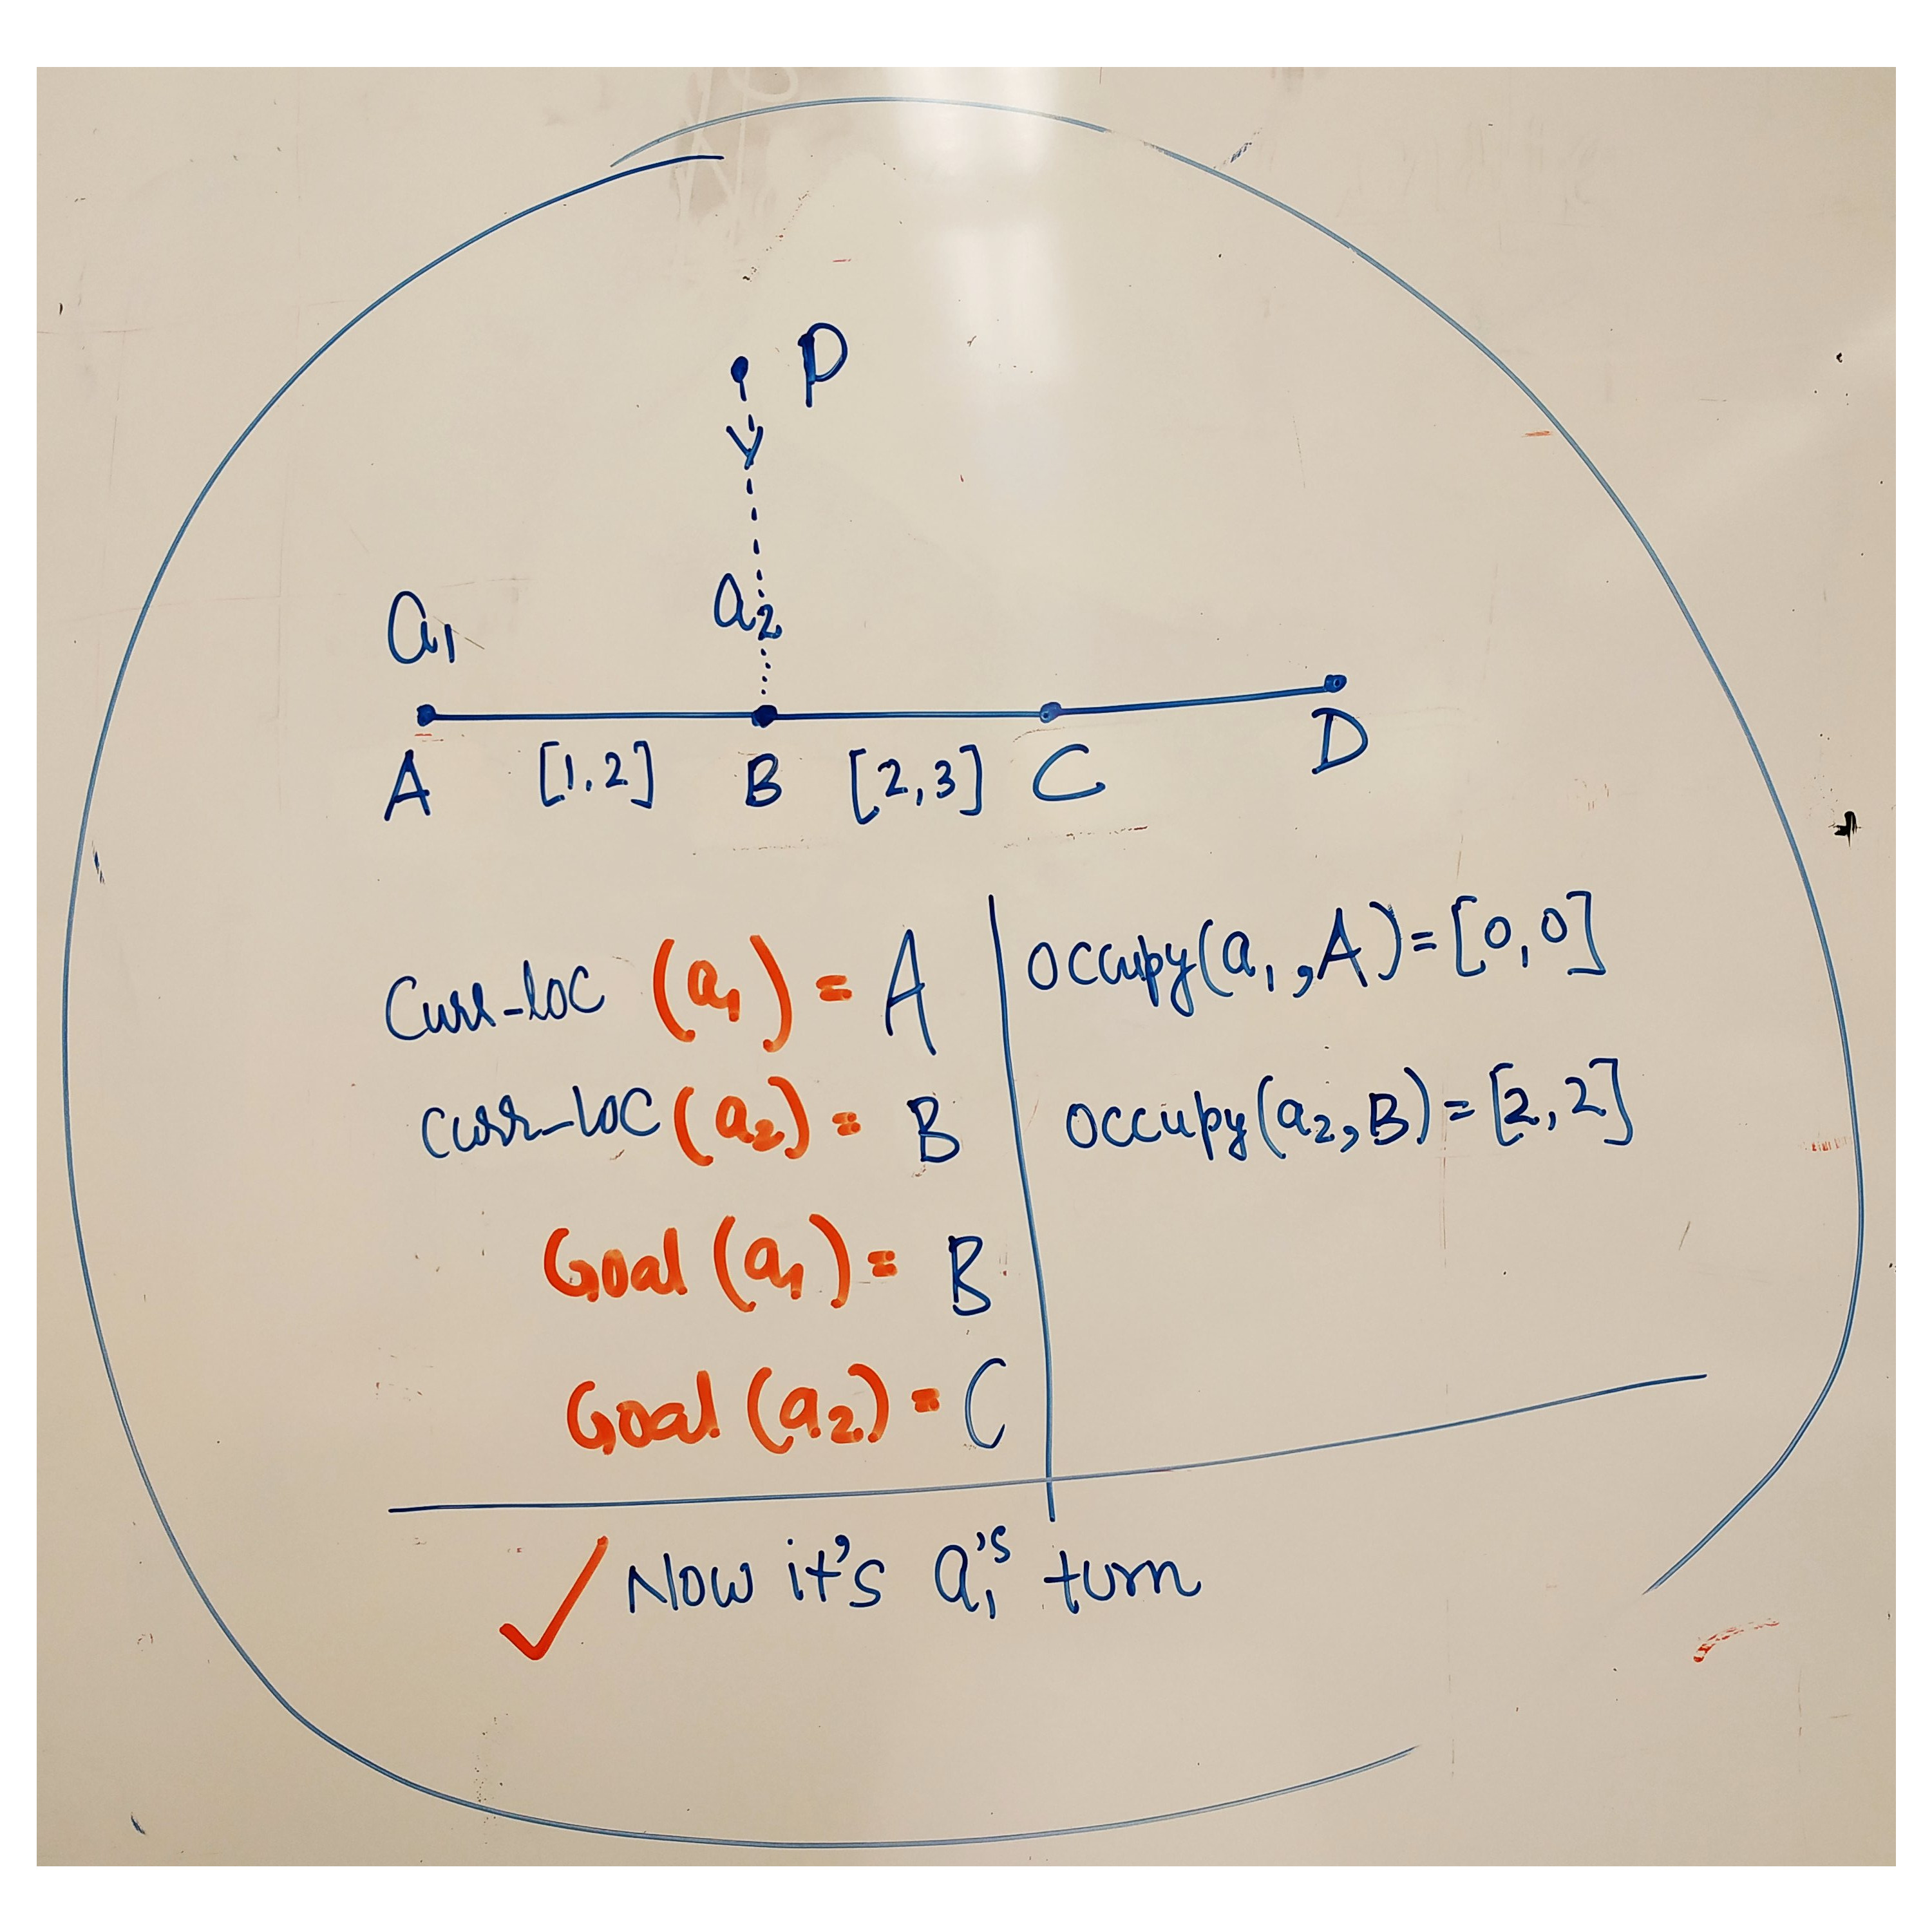
\includegraphics[width=7cm,height=7cm]{canvas.jpg}
    \caption{Example: $\mathrm{A^*+OD}$ under Time Uncertainty}
    \label{fig-aodtu}
\end{figure}

\section{MAPF under Uncertainty}
In this section we consider the complete uncertainty we propose in the new MAPF setting. 
We extends CBSTU and AODTU algorithms, described in the last section, to capture scenarios when agents have uncertainty about initial states and goal states too apart from the uncertainty in edge traversal times.  

\subsection{Conformant CBS under Time Uncertainty}
CCBSTU extends the explanation of CBSTU algorithm to handle a case when agents are not certain about their initial states and goal states. 
An agent maintains belief states over possible initial states and possible goal states. 
%
%CBSU algorithm is developed upon the extension of CBS algorithm discussed in the last section which covers only time uncertainty. 
%
%
Pseudo code to handle this MAPF setting is shown in Algorithm~\ref{algo.ccbstu} that implicitly captures the required pseudo code for CBSTU explained in the last section.
%
% In the basic CBS algorithm, an agent starts from one certain location called initial state (Sharon et el., 2012). 
% In many real world scenarios, agents might not be certain about their starting positions. 
%We adapt CBSTU algorithm that is an adaptation of the basic CBS algorithm. 
%We discuss an approach to find and resolve a conflict when non-deterministic finish time is considered along with an agent maintains an initial belief state and not a defined initial state.   
%The techniques used in the CBSTU algorithm to find a conflict for a given pair of paths and to resolve a conflict, remain the same in CCBSTU. 
%
%


\begin{algorithm}[h]
  \SetAlgoLined
  \KwData{An \emph{mapf} instance; An optimization function, $f$}
  \KwResult{\emph{conf-solution}~~~\textcolor{red}{// a conformant solution}}
  $root.constraints$ = $\phi$ \\
  $root.solution$ $\leftarrow$ individual \emph{conf-paths}       returned by \emph{bottom-level}() approach \\
  $root.cost$ = 
   		$\sum_{a_i \in {a_1,...,a_k}}
   			\sum_{\pi_i \in \Pi_{a_i}} f(\pi_i)$ \\
   
  ADD \emph{root} to OPEN \\  
  \While{OPEN not empty}
  {
  	$N$ $\leftarrow$ the best node from OPEN \\
  	Validate \emph{conf-paths} in $N$ until the first conflict occurs \\
  	\If{no conflict found}{
    	\textbf{return} $N$.$\emph{conf-solution}$ \\
    }
    $\emph{conflict}$ 
    		$\leftarrow$ First conflict  ~~~\textcolor{red}{// either vertex or edge} \\
    \For{agent $a_i$ $\in$ conflict}
    {
    	$A$ $\leftarrow$ \emph{Create} a new CT node \\
        \If{vertex-conflict$($conflict$)$}
        {
        	$A.constraints$ $\leftarrow$ $N.constraints$ + $(A,T_A,B,T_B,V)$ \\
        }
        \Else
        {
        	$A.constraints$ $\leftarrow$ $N.constraints$ + 
            	$(A,B,e_{com},[S_A+C_A,E_A+D_A],[S_B+C_B,E_B+D_B], [C_{com},D_{com}])$ \textcolor{red}{//~irrespective of the edge conflict types} 
        }
        
        $A.solution$ $\leftarrow$ $N.solution$ \\
        \emph{Update} $A.solution$ with a \emph{conf-path} 
         	returned by \emph{bottom-level}$()$ for $a_i$\\
        $A.cost = \sum_{a_i \in {a_1,...,a_k}}
   			\sum_{\pi_i \in \Pi_{a_i}} f(\pi_i)$ \\
        ADD node $A$ to OPEN \\    
    }
  }   
  \caption{The top-level CCBSTU approach.}
  \label{algo.ccbstu}
\end{algorithm}

The term \emph{conformant} is used by the planning community when an agent has no sensing capability and has uncertainty over its current position. We adapt this term in our explanation although we also have uncertainty about agents' goal locations. We change the definition and also the way CCBSTU now \emph{processes} a node of Constraint Tree (CT). 
%
%\subsection{Conformant CBSTU Algorithm}
%We discuss the main CCBSTU algorithm. 
%The pseudo code for the top-level approach is shown in Algorithm~\ref{algo.ccbstu}. The time intervals have been referred from Figure~\ref{fig:1}.
% that uses the previously discussed techniques to find out and resolve a conflict present in a node $N$ of a Constraint Tree (CT).

\noindent \subsubsubsection{\textbf{Definition of CCBSTU:}} 
%\noindent \textbf{Definition of CBSU:} 
We use the term \emph{conf-path} (conformant-path) only in the context of single-agent and \emph{conf-solution} (conformant-solution) to denote a set of $k$ conf-paths for a given set of $k$ agents. A conf-path for an agent $a_i$ is a set of paths $\Pi_{a_i}$. 
This set contains a single regular path -- the one described in CBSTU approach when we have only time uncertainty, for each possible initial location $l \in b_{I}^{a_i}$ and a possible goal location $g \in b_{g}^{a_i}$. 
%%
The rest of the details remain the same as in CBSTU algorithm (Section~3). Agents are associated with \emph{constraints} while they pursue their goals. A conf-path for an agent $a_i$ is \emph{consistent}, if each path $\pi_{a_i} \in \Pi_{a_i}$ is consistent with all $a_i$'s constraints. 
%
Similarly, a \emph{consistent} conf-solution is a solution that is made-up of such consistent conf-paths for individual agents. A solution is a \emph{valid} solution when all its $k$ conf-paths have \emph{zero} conflict.
The solution becomes invalid if there exists a path $\pi_{a_i}^l \in \Pi_{a_i}$, for an agent $a_i$, such that $\pi_{a_i}^l$ is inconsistent with any path $\pi \in \Pi_{a_j}$, where $a_i \neq a_j$.
%
A consistent conf-solution can be \emph{invalid} even if it consists of \emph{consistent} conf-paths but there exists a \emph{conflicting} pair of paths ($\pi_{a_i}$,$\pi_{a_j}$). 
%

The CCBSTU algorithm grows a set of constraints for each agent as search in CT progresses, and finds a conf-path that is consistent with their
individual constraints. 
For a given node of CT, a pair of conflicting paths makes a conf-solution inconsistent and the node of the CT is \emph{invalid}, and the conflict is marked which needs to be resolved. This node is declared as a \emph{non-goal} node.
The agent that receives a new constraint in the processing phase, must generate a new conf-path satisfying all their constraints. The algorithm works at two levels, at top, conflicts are found and constraints are generated and added, and at bottom, each agent generates a conf-path satisfying their constraints. 

\subsubsection{Top-Level: Search the Constraint Tree}
The algorithm searches a \emph{constraint tree} (CT) that is a binary tree. Each node $N$ of this tree contains the following things.  
\textbf{A set of constraints} ($N.\mathbf{constraints})$, that is empty for the root node of CT. Like CBSTU algorithm (Section~3), each child inherits all its parent's constraints, further it adds  exactly one new constraint for exactly one agent. \textbf{A conf-solution} ($N\mathbf{.conf\textnormal{-}solution})$, that is a set of $k$ consistent conf-paths -- one conf-path for each agent, found by the bottom-level approach. \textbf{The total cost} ($N\mathbf{.cost})$, that is $\sum_{a_i \in \{a_1...a_k\}} \sum_{\pi \in \Pi_{a_i}} \emph{LTB}(\pi)$. They are shown in the Algorithm~\ref{algo.ccbstu} (in Line~1,~2,~and~3).

\vspace{0.05in}
\noindent \subsubsubsection{\textbf{Processing a node}} 
%\noindent \textbf{Processing a node:} 
The \emph{bottom-level} approach is invoked in this phase which generates a shortest conf-path for each agent in a decoupled manner, such that all their individual constraints are satisfied in the process, i.e., each generated conf-path is consistent. 
Then, each agent's conf-path gets validated with every other agents' conf-paths. Unlike the CBS and CBSTU algorithms, this validation is a bit non-trivial. 
In this process, each $\pi_{i} \in \Pi_{a_i}$ is validated against each $\pi_{j} \in \Pi_{a_j}$ for all $j$ s.t. $j \neq i$. But the validation technique of a pair of paths remains the same as it was for CBSTU. If there is no conflict found, the node $N$ is declared a \emph{goal} node. Later, $N\textbf{.conf-solution}$ is returned. 
However, during the path validation, suppose that for two agents $a_i$ and $a_j$ and their paths $\pi_{i} \in \Pi_{a_i}$ and $\pi_{j} \in \Pi_{a_j}$, $(\pi_i,\pi_j)$ forms a conflicting pair, a new conflict is found in that case. 
The conflict could be either a vertex conflict or an edge conflict. 
We halt the validation process just after the very first conflict is found, and mark $N$ a \emph{non-goal} node.

\vspace{0.05in}
\noindent \subsubsubsection{\textbf{Resolving a conflict}
%\noindent \textbf{Resolving a conflict:}
We use different representations for edge and vertex conflicts in the CBSTU and CCBSTU algorithms. 
That means CCBSTU finds and resolves a conflict in exactly same way as CBSTU does. We have already discussed an approach to find and resolve a conflict. 
%
Given a new non-goal node $N$ of CT -- for which $N.\textbf{solution}$ contains a conflict that either arises due to an edge conflict: $(A,B,e_{com},[S_A+C_A,E_A+D_A],[S_B+C_B,E_B+D_B], [C_{com},D_{com}])$ or a vertex conflict: $(A,T_A,B,T_B,V)$.
The agents A and B are referred from Figure~\ref{fig:1}.
%%%
% We know that in any valid conf-solution as per our assumptions, at most one agent (either $a_i$ or $a_j$) is allowed to occupy a node or an edge at a time. 
Following our earlier discussion, CCBSTU generates two new children (in Line~13, Algorithm~\ref{algo.ccbstu}). In the first child a new constraint is added for agent $a_i$, and vice-versa for $a_j$ in the second child.   
At each new child, \emph{bottom-level} search is invoked only for the agent that gets the new constraint. The conf-paths for other agents remain the same, and can be inherited directly from parent node, $N$ in CT (in Line~21, Algorithm~\ref{algo.ccbstu}). 

\subsubsection{Bottom-Level: Find a New Conformant Path}
This is invoked to find a new conf-plan, only for the agent $a_i$ that received new constraints. 
It must find a new conf-path (if there exists one) such that it satisfies all the $a_i$'s constraints. 
The new conf-path is obtained independently, in a decoupled manner. 
An important consideration is that each agent maintains an initial belief state $b_{0}^{a_i}$ - a set of possible initial locations, such that each \emph{pair} of their belief states is \emph{disjoint}. 
For each location $l \in b_{0}^{a_i}$ and a definite goal location, any single-agent path finding algorithm can be adapted and used. For this location $l$ a solution, $\emph{path}_l$, is found in exactly the same way as it is done in the CBSTU algorithm. It stores each $\emph{path}_l$ in $\Pi_{a_i}$, and returns $\Pi_{a_i}$ in the end.    

\subsection{A$^{*}$ + OD under  Uncertainty}
We now describe CAODTU algorithm that is applied when agents have uncertainty about initial state, goal state and edge traversal time. We generalize the AODTU algorithm explained in the last section.

Suppose that there are $k$ agents $a_1, \ldots, a_k$ where each agent maintains a belief state containing possible initial states, $m_i$ possible locations in the graph, and a belief state containing possible goal states, $n_i$ possible locations. 
We transform this MAPF problem to a MAPF problem that has only uncertainty over edge traversal time. The transformed problem can be solved by the AODTU algorithm. 
From the original problem, we create a new problem containing $k \times m_i \times n_i$ agents with their definite initial states and goal states. 
Apart from this we also maintain $k$ different \emph{classes} of agents, which suggests that all $m_i \times n_i$ agents belong to one class (\emph{class-i}). We run the exact AODTU algorithm described earlier. 
Perhaps the only difference is that any two agents belonging to one class will never collide with each other (trivial). 
Therefore an agent belonging \emph{class-i} can have a potential conflict with another agent only if the latter belongs to a different class, say, \emph{class-x}. 
A solution obtained by an agent that belong to \emph{class-i}, is a valid solution if it has no conflict with the current solution of each agent of the remaining classes.  
The AODTU algorithm finds a solution for this transformed problem. The individual solutions of the agents belonging to one particular class form a conformant solution (\emph{conf-solution}) as described in the CCBSTU algoritm. 
This is a trivial generalization as there is just one agent in each class when there is no uncertainty over their initial states and goal states. In a general approach, when AODTU is run, it looks for a potential inter-class conflict irrespective of how many agents belong to one particular class.

\section{Theoretical Analysis}
The proposed algorithms strive for a strong solution for the MAPF problem under given uncertainty. We prove that CCBSTU and CAODTU always find an optimal solution if there exists one. We also prove that the proposed algorithms are sound and complete. 
We begin with the CCBSTU algorithm, while the later part of the section contains some important theoretical properties of the CAODTU algorithm.

\subsection{CCBSTU: Soundness and Completeness}
First, we provide with several supporting claims.
\begin{definition}
For a given node $N$ in a constraint tree, suppose $CV(N)$ be the set of all solutions for CBSTU (conf-solutions for CCBSTU) that are: (1) consistent with set of constraints of $N$ and (2) are also valid (i.e., without conflicts). 
\end{definition}
If $N$ is not marked as goal node, the $N.\mathbf{solution}$ ($N.\mathbf{conf\textnormal{-}solution}$) will not be in $CV(N)$ as it is not valid.

% Following our previous description related to Definition~1, if $N$ is not a goal node, a solution (a conf-solution) available at $N$ is not a part of $CV(N)$ as it is not valid.
\begin{definition}
For any solution $p \in CV(N)$ for CBSTU (conf-solution for CCBSTU), we say that node $N$ permits the solution (conf-solution for CCBSTU) $p$.
\end{definition}

The cost of a \emph{solution} (\emph{conf-solution} for CCBSTU) in $CV(N)$ is the sum of the costs of individual agents. 
Let $minCost(CV(N))$ be the minimum cost over all solutions (conf-solutions) in $CV(N)$, which is \emph{minimized} over all the solutions (conf-solutions), such that for a \emph{solution} the cost is $\sum_{a_i \in {a_1,...,a_k}} \emph{LTB}(\pi_{a_i})$ 
(for a \emph{conf-solution} the cost is $\sum_{a_i \in {a_1,...,a_k}} \sum_{\pi_i \in \Pi_{a_i}} \emph{LTB}(\pi_i)$).

\begin{lemma}
When optimizing on the earliest reaching time (LTB), the cost of a node $N$ in the CT is a lower bound on $minCost(CV(N)).$ 
\end{lemma}
\begin{proof}
In both CBSTU and CCBSTU algorithms, $N.\mathbf{cost}$ is the optimal cost for a set of paths (conf-paths for CCBSTU) that satisfies all the constraints for the agents at $N$.  
The set of paths (conf-paths) is consistent but does not necessarily to be a valid solution (conf-solution).
Therefore, $N.\mathbf{cost}$ is the lower bound on the cost of any set of paths (conf-paths) that make a valid solution (conf-solution for CCBSTU) for $N$. 
This is because no agent in any solution (conf-solution for CCBSTU) can achieve their goal sooner than this. 
\end{proof}
%%%%%
\begin{lemma}
The CBSTU algorithm returns an optimal solution while the solution obtained is optimized over the least reaching time (LTB).
\end{lemma}
\begin{proof}
Suppose that the high-level search in CT is about to expand the goal node $G$ next. Which means that all the valid solutions must be allowed by at least one node in OPEN. This statement is quite trivial to prove. Suppose that parent node ($N$) of the goal node ($G$) is chosen to be expanded, which also means $N$ does not carry a valid solution. Let us say it generates two nodes $N_1$ and $N_2$, and they get added to OPEN. For sure at least one of $N_1$ and $N_2$ must be $G$ as it must be satisfying the new constraint.

By Lemma~1, we say that if $p$ is a valid solution and node $N$ in OPEN allows this solution $P$, the following relation holds: $cost(N(p)) \leq cost(p)$. As we use the best-first approach in the high-level search, the cost of a goal node $G$ will the lower bound on $cost(N(p))$ and $cost(p)$.  
\end{proof}
%

Under the assumptions made by us in this work, a valid solution is required to be strong (\emph{i.e.}, robust) \emph{w.r.t.} all uncontrollable action durations. We need to make sure that all agents reach their goal locations without any collision, over all possible executions, despite run-time choices made by the nature.

\begin{lemma}
The CBSTU algorithm returns a strong solution.
\end{lemma}
\begin{proof}
We state that a valid solution obtained by CBSTU is not strong. Hence there exists at least one time instance ($t$ - an integer) that belongs to an edge traversal time range ($[T_{min},T_{max}]$), and $t \in [T_{min},T_{max}]$ can be chosen by the environment such that the solution is not collision free. 
By proof of contradiction our statement does not hold. With this we also proved that the CBSTU algorithm is sound.    
\end{proof}
%

\begin{lemma}
The CBSTU algorithm is  complete. 
\end{lemma}
\begin{proof}
The algorithm returns a strong solution. The completeness property guarantees that the algorithm must find a solution if there exists one.

We prove this lemma by the Principle of Mathematical Induction. \emph{Base step}: suppose the root node of the CT is the solution node. This node has \emph{no conflict}. The planner finds a collision free path for each agent. \emph{Induction step}: suppose that a branch of CT is followed unto depth $i$, for a node $N$, there is \emph{only one} remaining conflict between the paths of two agents $a_i$ and $a_j$. 
%%
At depth $i+1$ this node would be picked by CBSTU and expanded such that two new nodes $N_1$ and $N_2$ will be generated and will be placed into OPEN. 
Following CBSTU, $N_1$ resolves this conflict by restricting $a_i$ at some time instance $t$, and vice-versa for $N_2$. One of $N_1$ and $N_2$ will be the only solution and the algorithm must select that from OPEN and expand it eventually. Therefore if there exists a solution CBSTU guarantees to find it.

\end{proof}

\begin{theorem}
The CCBSTU algorithm is  complete.
\end{theorem}
\begin{proof}
By Lemma~4, we prove that CBSTU is complete when there is uncertainty over edge traversal times. Perhaps the CCBSTU algorithm that extends CBSTU, also deals with uncertainty over agents' initial and goal states.

A simple extension of the proof of Lemma~4, helps prove this. In the \emph{base case}, the root node will have a conformant path for each agent (captures a solution path for each combination of possible initial and goal states of that agent).
In the \emph{induction step}, at a depth $i$, a node from OPEN is selected that has only one conflict remaining. Logically, its expansion leads to the only possible solution and the search approach must find it.  
Note that the approach CCBSTU employs to find and resolve a conflict is the same as in CBSTU. 
Therefore to resolve this conflict $N_1$ and $N_2$ will be generated and will be placed into OPEN. The search process eventually selects the solution node (one of $N_1$ and $N_2$).
\end{proof}
%
\begin{theorem}
The CCBSTU algorithm always returns a solution that is always strong and conformant-optimal.
\end{theorem}
\begin{proof}
Use Lemma~3 and Lemma~4
\end{proof}

\subsection{CAODTU: Soundness and Completeness}
First, we provide with some supporting claims.
\begin{lemma}
A move of an agent verified with ValidMove is conflict free.    
\end{lemma}
\begin{proof}
Suppose that a \emph{move} gets validated by ValidMove call and it causes some conflict. Which means the move the agent made allows it to occupy a vertex or an edge at some specific time with at least one more agent. 
Algorithm~\ref{fig-aodtu} guarantees that the current move taken by an agent does not enable the agent to occupy an edge or a vertex already occupied by some other agent. Therefore our assumption does not hold.  
\end{proof}

\begin{theorem}
The CAODTU algorithm is sound and complete.
\end{theorem}
\begin{proof}

\end{proof}

\begin{theorem}
The CAODTU algorithm returns an optimal solution (like CCBSTU returns a conformant optimal solution).
\end{theorem}
\begin{proof}

\end{proof}

\section{Experimental Results}

\subsection{Environment}

We experimented with 
two DAO maps [[TODO: WHICH MAPS?]] 
from Stutervant's movingai repostiory [[TODO: URL]], 
a $8\times 8$ open grid,
a $32\times 32$ maze-like map. 


To introduce uncertainty over edge traversal time we use a parameter $U$. 
For every edge we set the min edge traversal time $e_l$ to be between $[1,1+U]$, chosen uniformely at random, 
and then the max edge traversal time is chosen uniformely from the range $[e_l,1+U]$.


We experimented with $U=1,2,3,4$
and number of agents $....$

The timeout was set to be 5 minutes. 


Expected results:

- Impact of $U$?
- Who is better and when: two version of A*, or CBS?
- Impact of number of agents
- Impact of type of map

\subsection{The Empirical Evaluation}

\section{Summary and Future Work}
We propose two new algorithms called CCBSTU and CAODTU that are based on, the CBS algorithm and $A^*$ with OD algorithm respectively, to solve the MAPF problem under proposed novel settings. For example, when path traversal time is indefinite and uncontrollable, and the agents are uncertain about their initial locations and goal locations. We provide thorough theoretical analyses for both the proposed algorithms, and showed scalability of the approaches empirically on new MAPF problems.

In future we intend to extend this work to handle scenarios when an edge has disjunctive traversal time uncertainties with uncontrollability, e.g., the edge traversal time belongs to $[T_{min_1},T_{max_1}] \cup [T_{min_2},T_{max_2}]$. Very recently researchers have looked upon having a problem deadline. For the given deadline, they look for a solution that maximizes the number of agents reaching their goal locations. In future we intend to introduce the notion of \emph{deadline} in our proposed MAPF problem. 
%In that case, an optimal approach would find a solution that  maximizes the number of agents reaching their goal locations without colliding with each other, with a minimum cumulative cost.
%% The file named.bst is a bibliography style file for BibTeX 0.99c
\bibliographystyle{named}
\bibliography{ijcai19}

\end{document}






% In one solution For the interval $[t_1,t_2]$, constraints on agent A are imposed and described as follows. Suppose, $t$ is the time when A and B occupy V simultaneously. One way to resolve this by restricting A using a constraint: {$(\neg move(A,e_A,t-D_A) \wedge \neg move(A,e_A,t-(D_A-1)) \wedge ... \wedge \neg move(A,e_A,t-C_A))$. Here, each component $\neg move(A,e_A,t_x)$ represents that A is not allowed to apply move action through edge $e_A$ at time $t_x$. Consequently, the conjunction removes all the possibilities for agent A occupying vertex V at time $t$. 
% For example, if A applies \emph{move} at $t-D_A$, at the earliest it can reach V by $t-D_A+C_A$ and late by $t$. Similarly, if A applies \emph{move} at $t-C_A$, at the earliest it can reach V by $t$ and late by $t-C_A+D_A$, and so on for intermediate values between $t-D_A$ and $t-C_A$. In all these cases there is possibility that A can occupy V at $t$. We generalize this approach for all $t \in [t_1,t_2]$. 
% This generalization under uncertainty and uncontrollability restricts A, following its current path, to occupy V in the interval $[t_1,t_2]$ in any situation that could occur, consequently allows agent B to execute its current plan as it is. 
% On the contrary, we can allow A to execute its current plan by restricting B in exactly the same way. This approach produces sound solutions as well as it is complete, and their proofs are formally covered later in the paper. 


%\subsubsection{CBSTU Algorithm}
We describe the CBSTU algorithm that uses the above discussed procedures to find out and resolve a conflict present in a node $N$ of a Constraint Tree (CT). 
Pseudo code to handle this MAPF setting is shown in Algorithm~\ref{algo.cbstu}.
%
%Note that in this section we strive to capture only time uncertainty. CBSTU is extended in the next section to capture uncertainty and partial observability about initial and goal states. 
\paragraph{Definition of CBSTU} 
We will use a term \emph{path} only in the context of single-agent and \emph{solution} to denote a set of $k$ paths for a given set of $k$ agents. 
Basically, one path for each agent in the solution. A path for an agent would be a sequence of vertices, in which each vertex associates to $[t_{min},t_{max}]$ that represents the time the agent could occupy this vertex following their path, e.g., for an agent starting from $I$ and the goal $G$, a path $\pi$ would look like: $I[0,0] \rightarrow C[3,6] \rightarrow E[4,7] \rightarrow T[5,9] \rightarrow G[6,10]$. 

Agents are associated with \emph{constraints} while they pursue their goals. A \emph{consistent} path for an agent $a_i$ is the path that satisfies all its constraints. Similarly, a \emph{consistent solution} is a solution that is made-up of consistent paths for all the agents. A solution is \emph{valid} if all its $k$ paths have no conflicts. 
A consistent solution can be \emph{invalid}, even if it consists of consistent paths based on agents' current constraints, if there exists a pair of conflicting paths.
The important aspect of CBSTU is to grow a set of constraints for each agent, and find a path that is consistent with their individual constraints. A pair of conflicting paths makes a solution invalid, and the conflict is \emph{marked} and gets resolved. 
The conflicting agents must generate new paths by satisfying all the constraints added after the previous conflict was resolved.
CBSTU works at two levels - top level and bottom level. 
At the top-level, conflicts are found and constraints are generated and added to the constraint list. 
At the bottom-level, each agent generates a new plan respecting their individual constraints. 
This is done in a \emph{decoupled} manner. Next, we discuss each part of the whole process in detail.

\subsubsection{Top-Level: Search the Constraint Tree}
The algorithm searches a \emph{constraint tree} (CT) which is a binary tree. Each node $N$ of this tree contains the following. 
\textbf{A set of constraints} ($N$.$\mathbf{constraints}$), that is empty for the root node of CT. Like the CBS algorithm, each child inherits the set of constraints of their parent. The approach adds exactly one new constraint in this set, exactly one for one agent. 
\textbf{A solution} ($N$.$\mathbf{solution}$), that is a set of $k$ consistent paths -- one for each agent, found by the bottom-level approach, discussed next. \textbf{The total cost} ($N$.$\mathbf{cost}$), that is $\sum_{a_i \in \{a_1...a_k\}} \emph{LTB}(\pi_i)$ (in Line 1, 2, and 3, in Algorithm~2). 
\emph{LTB} of a path represent the lowest time the agent takes to reach the goal. In the previous example, $\pi$ ($I \rightarrow C \rightarrow E \rightarrow T \rightarrow G$) has \emph{LTB$(\pi)$} $= 6$. 
For an edge they capture the lower time bound, an agent could occupy the edge during traversal starting from their initial location. 
For $\pi$, $\emph{LTB}(E-T)$ is $5$. Similarly, for a vertex in a given path, it show the lower time bound an agent can occupy a vertex, e.g., $\emph{LTB}(E)$ is $4$.  

%Note that for an edge $e$ in the graph $\graph$, we consider that the Lowest Traversal Time, $\emph{LTT}(e) \geq 1$. The Highest Traversal Time, $\emph{HTT}(e)$, is bounded by some value, say LARGE, s.t., $\emph{HTT}(e) \geq \emph{LTT}(e)$.

\paragraph{Processing a Node of CT} In this phase of the algorithm, the bottom-level approach is invoked. This approach generates a shortest path for each agent independently, such that all their individual constraints are satisfied in the process, i.e., each generated path is consistent \emph{w.r.t.} the constraints. 
Once this is done, the path of one agent gets validated with the paths of every other agents. If there is no conflict found, the node $N$ is declared a \emph{goal} node. $N$ contains agents individual consistent paths, therefore $N.\mathbf{solution}$ is returned. 
However, during the path validation, suppose two agents $a_i$ and $a_j$ have their paths conflicting, the approach to find such a pair of paths is discussed earlier section. It finds a new conflict that could be either associated to a vertex conflict or an edge conflict (a head-on or run-over case). The validation process halts just after the very first conflict is found, and marks $N$ a \emph{non-goal} node.

%\subsubsection{Resolving a Conflict}
\paragraph{Resolving a Conflict}
Given a new non-goal node $N$ whose \emph{solution} contains an conflict $\emph{conflict}$ that either arises due to an edge conflict: $(A,B,e_{com},\tau(\pi_A,e_{com}),\tau(\pi_B,e_{com}), [C_{com},D_{com}])$ or a vertex conflict: $(A,\tau(\pi_A,V),B,\tau(\pi_B,V),V)$.
%
As per our assumptions, at most one of A and B is allowed to occupy a vertex or an edge at a given time. Therefore, for each conflict, $N$ produces two new children (Line 13, Algorithm 2), which are examined independently to maintain optimality. 
One child adds a new constraint for agent A following the conflict resolution step. Similarly, it is done for agent B, in the other child of $N$. 
In the new children, the bottom-level search should be invoked only for the agent that receives the new constraint. 
The paths of the remaining agents will be the same and they are inherited without any modifications (Line 21, Algorithm 2).

For ease of exposition we consider a pair of two agents given their individual paths, to find conflicts.



Since we have explicit notion of time ranges, applying actions in a round-robin fashion~\cite{Standley10} may generate an illegal solution.
Explicit time in the representation could help an \emph{ordered} agent to occupy a location far ahead in future. This location could be the goal location for the next agent. 
Once the next agent reaches its goal it can wait for indefinite time. This might be not trivial to detect. 
In figure~\ref{oda-fail}, agent $a_2$ is at its goal location ($G_2$) which is also its initial location ($S_2$) and agent $a_1$'s goal is $G_1$ and its initial location is $S_1$. 
If a round-robin ordering is followed, say $a_1$ is followed by $a_2$. 
The search begins, $a_1$ moves to $S_2$ and occupies it at $[10,10]$. Next, $a_2$ waits at its goal, since it is already at its goal location, consequently the resulting state would be $\langle \langle a_1, S_2, T_1 = [10,10] \rangle, \langle a_2, S_2, T_2 = [1,1] \rangle \rangle$. 
In the same way $a_1$ again moves to $G_1$ and $a_2$ waits at $G_2$, resulting in a goal state, $S_G = \langle \langle a_1, G_1, T_1 = [11,11] \rangle, \langle a_2, G_2, T_2 = [2,2] \rangle \rangle$. 
All moves taken til this point are the valid as per \emph{ValidMove} (Algorithm~\ref{algo.validateMove}) but the goal state is illegal.

\begin{figure}
    \centering
    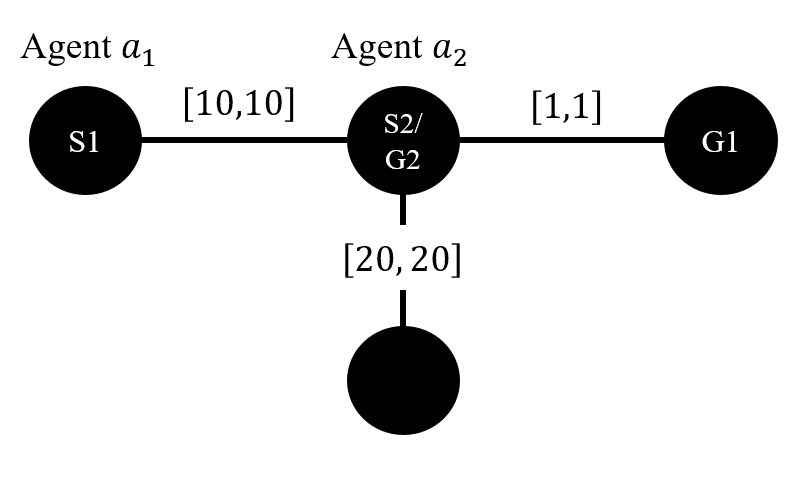
\includegraphics[width=6cm,height=3.5cm]{oda-graph.png}
    \caption{A$^*$ with OD - where the round robin approach fails}
    \label{oda-fail}
\end{figure}

%This is true even if some agents are yet to apply their actions to finish with the current ordered sequence. 
%

%Our algorithm maintains two conceptually different types of states. They are \emph{standard} state -- in which no agent is assigned an operator, and \emph{intermediate} state -- in which there exists an agent with an assigned operator. 
%
%Assigning a move to the last unassigned agent in an intermediate state results in a standard state. A$^*$ treats these states equivalently and hence they can be expanded in any order. 

%Once an arbitrary ordering is decided then $A^*$ is run.



\begin{figure}
    \centering
    %\begin{subfigure}
        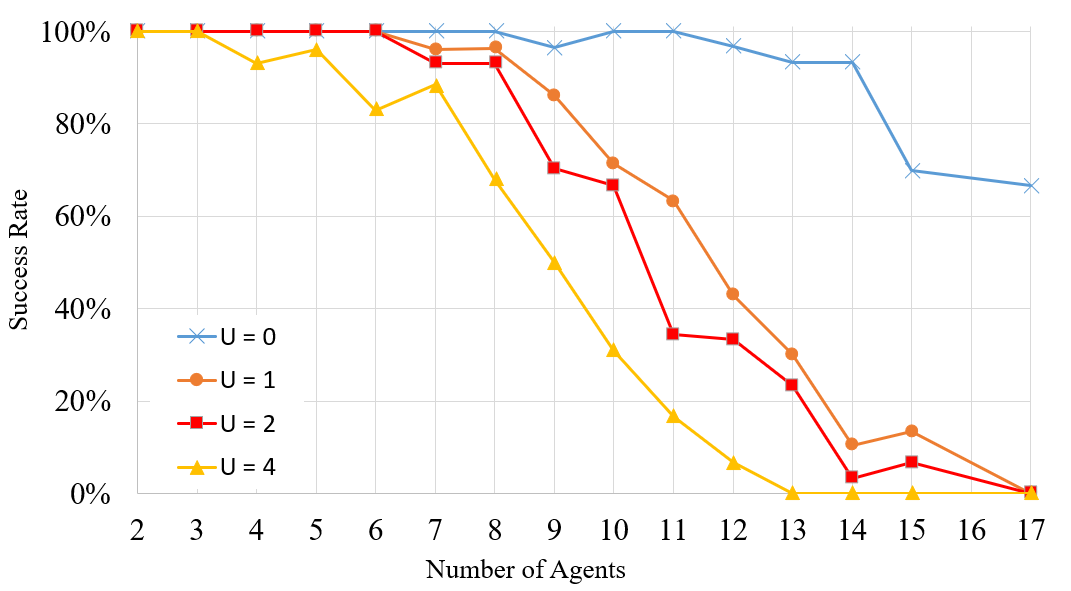
\includegraphics[width=0.48\textwidth]{CBS.png}
    %\end{subfigure}
    %\begin{subfigure}
        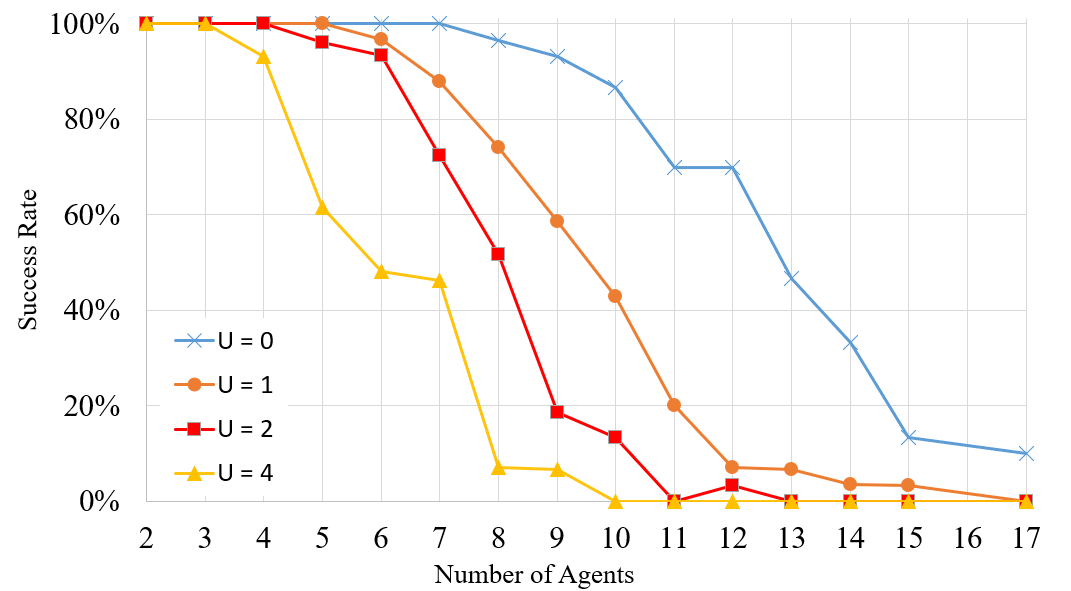
\includegraphics[width=0.48\textwidth]{ODA.png}
    %\end{subfigure}
    \caption{\emph{Success rate} of CBSTU (top) and ODATU (bottom) for a fixed  number of agents and uncertainty parameter ($U$).}
    \label{succ-rate-oda-cbs}
\end{figure}






In classical MAPF, there are two common solution cost functions: sum-of-costs and makespan. 
For a 
In MAPF-TU, there are a 
A MAPF-TU instance may have several solutions, and some of them might be preferable to others. 
Under the overarching sum-of-cost objective



measures, but we take the following simple app


generic approach: first, we choose between adopting an optimistic or pessimistic view with regards to how the time uncertainty is resolved; second we compute for each agent an individual cost, and finally we aggregate the cost across the paths for all agents.
%For instance, in certain scenarios we may aim to minimize the arrival time of the latest agent whereas in other scenarios it is the total time spent across all agents that needs to be minimized. 

Drawing inspiration from the field of computational social choice and resource allocation, we highlight the \emph{utilitarian} and \emph{egalitarian} aggregation functions.
The utilitarian perspective tends to be used when efficient solutions are important~\cite{ChevaleyreELM2007}, for instance, if the agents were robots and we wanted to minimize the total energy spent  executing the plan; in this case, it is the total time spent across all agents that needs to be minimized.
On the other hand, the egalitarian perspective can be used when fair solutions are prioritized, for instance, if the agents were delivering goods to customers and we wanted to avoid having any customer waiting for too long.
In that case, we may aim to minimize the arrival time of the latest agent.


\begin{definition}
Let $\tuple{\vertices, \edges, \timel, \timeu, \sourcetargets}$ be a MAPF-TU instance with $k$ agents, and let $\Pi = (\vertexpath_1 = v_0^1\dots v_{n_1}^1$, \dots, $\vertexpath_k = v_0^k\dots v_{n_k}^k)$ be a strong solution.
The \emph{optimistic} individual cost for agent $i$ is $c_i = \sum_{0 \leq j < n_i} \timel(v_j^i, v_{j+1}^i)$ whereas the \emph{pessimistic} individual cost for agent $i$ is the same computation using $\timeu$ in place of $\timel$.
The \emph{utilitarian} collective cost of $\Pi$ is $\sum_{1 \leq i \leq k} c_i$  whereas the \emph{egalitarian} collective cost of $\Pi$ is $\max_{1 \leq i \leq k} c_i$.
\end{definition}








To that end, we use a modified version of the low-level solver of the CBSTU algorithm which can search a new path. 
%while adhering to a given set of constraints. 
In order to ensure that agents will not collide with each other despite planning independently, $a_i$ must restrict its future moves such that it can only search along the vertices and the edges that comprised $\pi_i$.
%i.e., the agent can only search along the vertices and the edges that comprised its original offline path. 
Roughly speaking, $C_{i}$ basically contains only the valid potential presences over those edges and vertices, and if $a_i$ takes a move such that its potential presence is not part of $C_i$, is invalid.
%
Hence, in principle, during replanning the search space for $a_i$ will be a small fraction of the original graph. 
%
%It consists of only the edges and vertices that are part of the original path, of course with the time restrictions imposed on them by $C_i$. 
%
The agent continues to execute once a new plan found, if exists.
This process continues for all the agent independently, until all the agents arrive at their goal locations.
\abda{I don't understand this. To me the replanning can only decrease the amount of waiting actions. Anything other than that sounds potentially unsafe to me (unless the offline planning has computed a lot of extra information beyond the paths and the potential presences, but that's complicated and we are not telling the reader how it's done). I don't see the need for a search space or anything complicated like that.}





\paragraph{Time Complexity}
%The algorithm consists of two phases --- each with a different time complexity.
Since MAPF-TU problem is a variant of the standard MAPF problem, finding an optimal, safe offline plan in the first phase of our online approach itself is exponential in time.
%In the first phase of finding a centralized offline plan is exponential in time as it is a variant of the standard MAPF problem.
\abda{we can be more precise than that: finding the centralized plan corresponds to solving MAPFTU, rather than MAPF. And the exponential needs of MAPFTU should have been discussed or evoked earlier.}
Once we generate all necessary constraints based on the initial offline solution, each replanning phase is polynomial time since the agents need to plan only for themselves. 
In practice, it is very fast since the search is performed on a small subset of the graph with a limited depth and branching factor. 
In the experiments, the time it takes to find an initial offline solution was significantly greater than the subsequent replanning stages.
